% MACURA: the paper and my racing-drone project (35 pages: Part I 18 slides, Part II 12 slides)
% Build:  latexmk -pdf macura_presentation.tex      (or: pdflatex macura_presentation.tex twice)
% figures/paper:   cropped from the paper (arXiv:2405.19014v3)
% figures/project: plots and video frames from the project (python3 paper/presentation/make_figures.py)
\documentclass[aspectratio=169,10pt]{beamer}

% ── edit these ────────────────────────────────────────────────────────────────────────────────────
\newcommand{\presenter}{Silver Gjeka}
\newcommand{\course}{}                       % e.g. \renewcommand{\course}{Reinforcement Learning -- }
\newcommand{\talkdate}{\today}

% ── packages ──────────────────────────────────────────────────────────────────────────────────────
\usepackage[T1]{fontenc}
\usepackage{amsmath,amssymb}
\usepackage{booktabs}
\usepackage{array}
\usepackage{graphicx}
\usepackage{algorithm}
\usepackage{algpseudocode}
\usepackage{tikz}
\usetikzlibrary{arrows.meta,positioning,shapes.geometric,calc}

% ── look ──────────────────────────────────────────────────────────────────────────────────────────
\definecolor{navy}{HTML}{1B2F5E}
\definecolor{mygreen}{HTML}{2E7D32}
\definecolor{myred}{HTML}{C62828}
\definecolor{myorange}{HTML}{EF6C00}
\definecolor{myblue}{HTML}{1565C0}
\definecolor{lightgray}{HTML}{EEEEEE}
\setbeamertemplate{navigation symbols}{}
\setbeamercolor{title}{fg=navy}
\setbeamercolor{subtitle}{fg=navy}
\setbeamercolor{frametitle}{fg=navy}
\setbeamercolor{structure}{fg=navy}
\setbeamercolor{normal text}{fg=black}
\setbeamercolor{itemize item}{fg=black}
\setbeamercolor{itemize subitem}{fg=black}
\setbeamercolor{enumerate item}{fg=black}
\setbeamercolor{caption name}{fg=navy}
\setbeamerfont{title}{series=\bfseries,size=\LARGE}
\setbeamerfont{subtitle}{series=\bfseries,size=\normalsize}
\setbeamerfont{frametitle}{series=\bfseries,size=\Large}
\setbeamerfont{caption}{size=\scriptsize}
\setbeamertemplate{itemize items}[circle]
\setbeamertemplate{itemize subitem}[circle]
\setbeamertemplate{enumerate items}[default]
\setbeamertemplate{frametitle}{%
  \vspace*{0.55em}\insertframetitle\par\vspace{0.1em}%
  {\color{navy}\rule{\linewidth}{0.5pt}}\vspace{-0.3em}}
\setbeamertemplate{footline}{%
  \hspace*{1.3em}{\scriptsize\color{gray}\insertsectionhead}\hfill\scriptsize\insertframenumber\,/\,\inserttotalframenumber
  \hspace*{1.3em}\vspace*{0.7em}}
\setbeamertemplate{caption}{\centering\insertcaption\par}

% a part divider: "Part N" + title + what it covers
\newcommand{\partslide}[3]{%
  \begin{frame}[plain]
    \vfill\centering
    {\large Part #1}\par\vspace{1.0em}
    {\usebeamerfont{title}\color{navy}#2\par}\vspace{1.0em}
    {\normalsize #3\par}
    \vfill
  \end{frame}}

% ── notation ──────────────────────────────────────────────────────────────────────────────────────
\newcommand{\Denv}{\mathcal{D}_{\mathrm{env}}}
\newcommand{\Dmod}{\mathcal{D}_{\mathrm{mod}}}
\newcommand{\E}{\mathcal{E}}
\newcommand{\ugjs}{u_{\mathrm{GJS}}}
\newcommand{\ptil}{\tilde{p}}
\newcommand{\chg}[1]{{\color{myorange}\bfseries #1}}                 % the line where a method differs
\newcommand{\code}[1]{{\scriptsize\color{gray}\texttt{#1}}}          % where it is in my code
\algrenewcommand\algorithmicrequire{\textbf{Given:}}
\algrenewcommand\algorithmiccomment[1]{\hfill{\color{gray}\(\triangleright\) #1}}

% ── TikZ styles ───────────────────────────────────────────────────────────────────────────────────
\tikzset{
  box/.style={draw, rounded corners=3pt, thick, align=center, minimum height=0.9cm, fill=lightgray,
              font=\small, inner sep=4pt},
  bluebox/.style={box, fill=myblue!12, draw=myblue},
  greenbox/.style={box, fill=mygreen!12, draw=mygreen},
  orangebox/.style={box, fill=myorange!14, draw=myorange},
  redbox/.style={box, fill=myred!10, draw=myred},
  arr/.style={-{Stealth[length=2.4mm]}, thick},
  lab/.style={font=\scriptsize, align=center},
}

\title{Trust the Model Where It Trusts Itself}
\subtitle{MACURA: the paper, and my project on a racing drone}
\author{\presenter}
\institute{\small Department of Computer Science\\ Master's Degree in Artificial Intelligence\\ University of Verona}
\date{\small \course\talkdate\\[0.8em]\scriptsize Paper: B.~Frauenknecht, A.~Eisele, D.~Subhasish, F.~Solowjow, S.~Trimpe
      (RWTH Aachen), ICML 2024, arXiv:2405.19014\\ Project code: github.com/silvergjeka22/macura-drone}

\begin{document}

\begin{frame}[plain]
  \titlepage
\end{frame}

\begin{frame}{Outline}
  \begin{columns}[T]
    \begin{column}{0.47\textwidth}
      {\large\bfseries\color{navy} Part I -- The paper}
      \begin{enumerate}
        \item The problem: when and where to trust a model
        \item Background: SAC, ensembles, Dyna, MBPO and M2AC
        \item MACURA: stop imagining where the model is unsure
        \item The four algorithms side by side
        \item Noise, results and what matters
      \end{enumerate}
    \end{column}
    \begin{column}{0.49\textwidth}
      {\large\bfseries\color{navy} Part II -- My project}
      \begin{enumerate}\setcounter{enumi}{5}
        \item The task: a racing drone with wind and a chute
        \item Implementation and a fair protocol
        \item Results: learning, testing, trust, one flight
        \item Limitations and conclusion
      \end{enumerate}
    \end{column}
  \end{columns}
\end{frame}

% ════════════════════════════════════════════════════════════════════════════════════════════════
\partslide{I}{The Paper}{How MACURA decides \emph{where} to trust its learned model}
\section{I \textperiodcentered{} Background}

% ── I.1 ───────────────────────────────────────────────────────────────────────────────────────────
\begin{frame}{The Problem: When and Where to Trust a Model}
  \begin{itemize}
    \item Deep RL needs \textbf{millions of interactions}. On a real robot or drone, each one is slow, expensive or
          risky.
    \item \textbf{Model-based RL} learns a model of the world and uses it to \textbf{imagine} extra experience.
    \item But a learned model is never perfect, and training on its \textbf{wrong predictions} misleads the agent.
  \end{itemize}
  \vspace{0.3em}
  \begin{columns}[T]
    \begin{column}{0.48\textwidth}
      \begin{block}{MBPO: \emph{when} to trust the model}
        Imagined trips get longer during training by a \textbf{hand-made schedule}, and the model is trusted
        \textbf{equally everywhere}.
      \end{block}
    \end{column}
    \begin{column}{0.48\textwidth}
      \begin{block}{MACURA: \emph{where} to trust the model}
        A model is accurate in some places and not in others, so every imagined trip \textbf{stops where the model
        itself becomes uncertain}.
      \end{block}
    \end{column}
  \end{columns}
  \vspace{0.4em}
  \small\textbf{Contributions of the paper}: (1) a guarantee of improvement inside a set $\E$ of accurate states;
  (2) a cheap uncertainty measure (GJS) to find $\E$; (3) adaptive imagined trips with essentially \textbf{one
  hyperparameter} $\xi$; (4) better results than MBPO and M2AC on MuJoCo.
\end{frame}

% ── I.2 ───────────────────────────────────────────────────────────────────────────────────────────
\begin{frame}{Background: SAC and Probabilistic Ensembles}
  \begin{columns}[T]
    \begin{column}{0.48\textwidth}
      \textbf{Soft Actor-Critic (SAC)}: the learner inside every method
      \begin{itemize}\small
        \item An \textbf{actor} (the policy) and \textbf{critics} that learn $Q(s,a)$, the expected future reward.
        \item \textbf{Maximum entropy}: it maximises reward plus randomness, so it keeps exploring:
              \[ J(\pi)=\textstyle\sum_t \mathbb{E}\big[r(s_t,a_t)+\alpha\,\mathcal{H}(\pi(\cdot\mid s_t))\big] \]
        \item Two critics (it takes the smaller value) and a temperature $\alpha$ that tunes itself.
        \item \textbf{Off-policy}: its target $r+\gamma Q(s',a')$ works on any stored transition, \textbf{real or
              imagined}.
        \item $G$ = gradient updates per real step (the \textbf{update-to-data ratio}).
      \end{itemize}
    \end{column}
    \begin{column}{0.48\textwidth}
      \textbf{Probabilistic ensemble}: the learned model
      \begin{itemize}\small
        \item $E=7$ neural networks, each trained on its own bootstrap sample of the real data.
        \item Each predicts the next state as a \textbf{Gaussian}: $\ptil_{\theta_e}(s'\mid s,a)=\mathcal{N}(\mu_{\theta_e},\Sigma_{\theta_e})$.
        \item \textbf{Aleatoric} uncertainty (the world is random) $\Rightarrow$ each network predicts a \textbf{wide}
              Gaussian.
        \item \textbf{Epistemic} uncertainty (too little data) $\Rightarrow$ the networks \textbf{disagree}.
        \item In an imagined trip, every step uses a \textbf{random} network.
      \end{itemize}
      \vspace{0.3em}
      \colorbox{myorange!12}{\parbox{0.95\linewidth}{\small Only epistemic uncertainty means ``the model may be
      \textbf{wrong} here''. MACURA is built on this difference.}}
    \end{column}
  \end{columns}
\end{frame}

\section{I \textperiodcentered{} Model-based RL}

% ── I.3 ───────────────────────────────────────────────────────────────────────────────────────────
\begin{frame}{Dyna-Style MBRL: Imagined Rollouts}
  \begin{columns}[T]
    \begin{column}{0.46\textwidth}
      \begin{figure}
        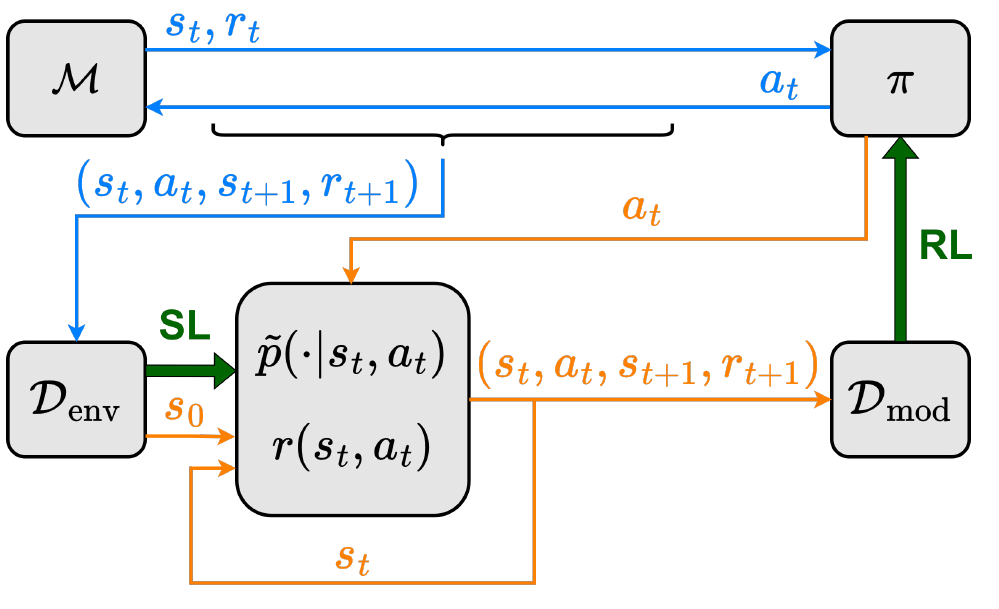
\includegraphics[width=\linewidth]{figures/paper/fig1_dyna.png}
        \caption{Dyna-style MBRL (paper, Fig.~1).}
      \end{figure}
    \end{column}
    \begin{column}{0.52\textwidth}
      \footnotesize
      \begin{itemize}
        \item \textcolor{myblue}{\textbf{Real world}} (blue): the policy $\pi$ acts in the real MDP $\mathcal{M}$; every
              transition is stored in the real buffer $\Denv$.
        \item \textcolor{mygreen}{\textbf{Learning}} (green): the model $\ptil$ learns from $\Denv$ by supervised
              learning (SL); SAC learns from the imagined data (RL).
        \item \textcolor{myorange}{\textbf{Imagination}} (orange): \textbf{branched rollouts} start from real states
              $s_0\in\Denv$ and imagine a few steps with $\pi$ and $\ptil$; the steps go to $\Dmod$. SAC trains on
              95\% imagined + 5\% real data.
      \end{itemize}
      \textbf{Why it helps}: much more training data per real step, and it follows the \textbf{current} policy.\\[0.3em]
      \textbf{The risk}: every imagined step builds on the previous prediction, so errors add up, and the agent learns
      the model's mistakes (\textbf{model exploitation}).\\[0.3em]
      $\Rightarrow$ The methods differ in \textbf{how far they imagine, and which imagined steps they keep}.
    \end{column}
  \end{columns}
\end{frame}

% ── I.4 ───────────────────────────────────────────────────────────────────────────────────────────
\begin{frame}{MBPO and M2AC: Two Earlier Answers}
  \begin{columns}[T]
    \begin{column}{0.4\textwidth}
      \textbf{MBPO} (Janner et al., 2019)
      \begin{itemize}\small
        \item Every imagined trip has the \textbf{same length} $k$. It grows during training by a \textbf{schedule}
              chosen by hand for each task (Humanoid $1\to25$, Walker 1).
        \item \textbf{Every} imagined step is used: the model is never checked.
        \item A \textbf{fixed} number $G$ of SAC updates per real step.
      \end{itemize}
      $\Rightarrow$ It answers \emph{when} to trust the model, not \emph{where}.
    \end{column}
    \begin{column}{0.56\textwidth}
      \textbf{M2AC} (Pan et al., 2020): masking by uncertainty
      \begin{itemize}\small
        \item It measures uncertainty \textbf{one-vs-rest (OvR)}: the network that made the prediction against a
              Gaussian fitted to the others.
        \item All trips run the full horizon $H$. At step $h$ it keeps only the share $\frac{H-h}{2(H+1)}$ with the
              \textbf{lowest} uncertainty: about 25\% of all steps.
        \item The rule is \textbf{rank-based}: it keeps the same share when all data are bad, and throws data away
              when all are good.
        \item A \textbf{reward penalty} $r-\alpha\,u$ pushes the agent away from uncertain regions, which can also
              slow exploration.
      \end{itemize}
    \end{column}
  \end{columns}
\end{frame}

\section{I \textperiodcentered{} MACURA}

% ── I.5 ───────────────────────────────────────────────────────────────────────────────────────────
\begin{frame}{Where to Trust Your Model?}
  \begin{columns}[T]
    \begin{column}{0.4\textwidth}
      \begin{figure}
        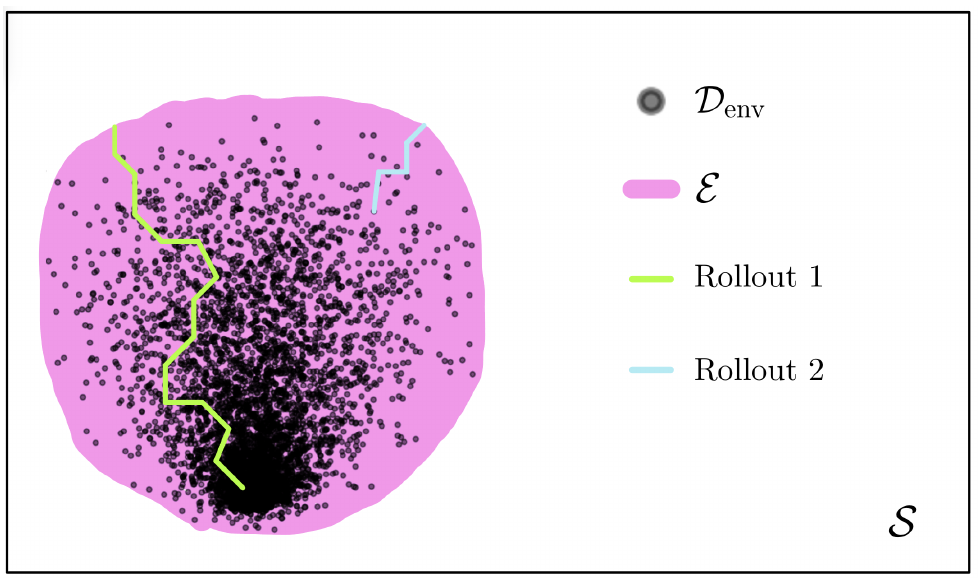
\includegraphics[width=\linewidth]{figures/paper/fig2_where.png}
        \caption{The real data define a set $\E$ where the model is accurate (paper, Fig.~2).}
      \end{figure}
    \end{column}
    \begin{column}{0.58\textwidth}
      \small
      \begin{itemize}
        \item Inside $\E$, long imagined trips are useful. Once a trip \textbf{leaves} $\E$, its data are harmful.
        \item Some trips stay in $\E$ for a long time, others leave it at once: \textbf{one fixed length cannot fit
              both}.
      \end{itemize}
      \textbf{Theorem 4.1} (simplified): if trips stop when they leave $\E$,
      \[ \eta[\pi]\;\ge\;\tilde\eta[\pi]-C,\qquad C=2r_{\max}\textstyle\sum_{t}\gamma^t\sum_{\tau\le t}\Delta p_{\E}[\pi] \]
      $\eta$ is the real return, $\tilde\eta$ the return in the model, and $\Delta p_{\E}$ the largest model error
      \textbf{inside} $\E$. If the policy improves in the model by more than $C$, it also improves in reality.\\[0.4em]
      \textbf{In practice} the real error is unknown, so $\E$ is estimated from the model's own uncertainty:
      \[ \E=\{\,s\mid u(s,a)<\kappa,\ a\sim\pi(\cdot\mid s)\,\} \]
    \end{column}
  \end{columns}
\end{frame}

% ── I.6 ───────────────────────────────────────────────────────────────────────────────────────────
\begin{frame}{GJS Uncertainty: Do the Networks Agree?}
  \small
  MACURA measures the average disagreement over \textbf{all pairs} of networks ($\mathcal{N}_e$ = network $e$'s
  Gaussian):
  \[
    \ugjs(s,a)=\frac{2}{E(E-1)}\sum_{e<f} D_{\mathrm{GJS}}(\mathcal{N}_e\|\mathcal{N}_f),\qquad
    D_{\mathrm{GJS}}=\tfrac12 D_{\mathrm{KL}}(\mathcal{N}_e\|\mathcal{N}_{ef})+\tfrac12 D_{\mathrm{KL}}(\mathcal{N}_f\|\mathcal{N}_{ef})
  \]
  where $\mathcal{N}_{ef}$ is the \textbf{geometric mean} of the two Gaussians (again a Gaussian).
  \begin{itemize}
    \item It has a \textbf{closed form} and is symmetric, so it is cheap enough for \textbf{every} imagined step.
    \item It is large when two networks are \textbf{confident but predict different things}, and zero when they predict
          the same wide Gaussian (pure noise).
  \end{itemize}
  \vspace{-0.3em}
  \begin{figure}
    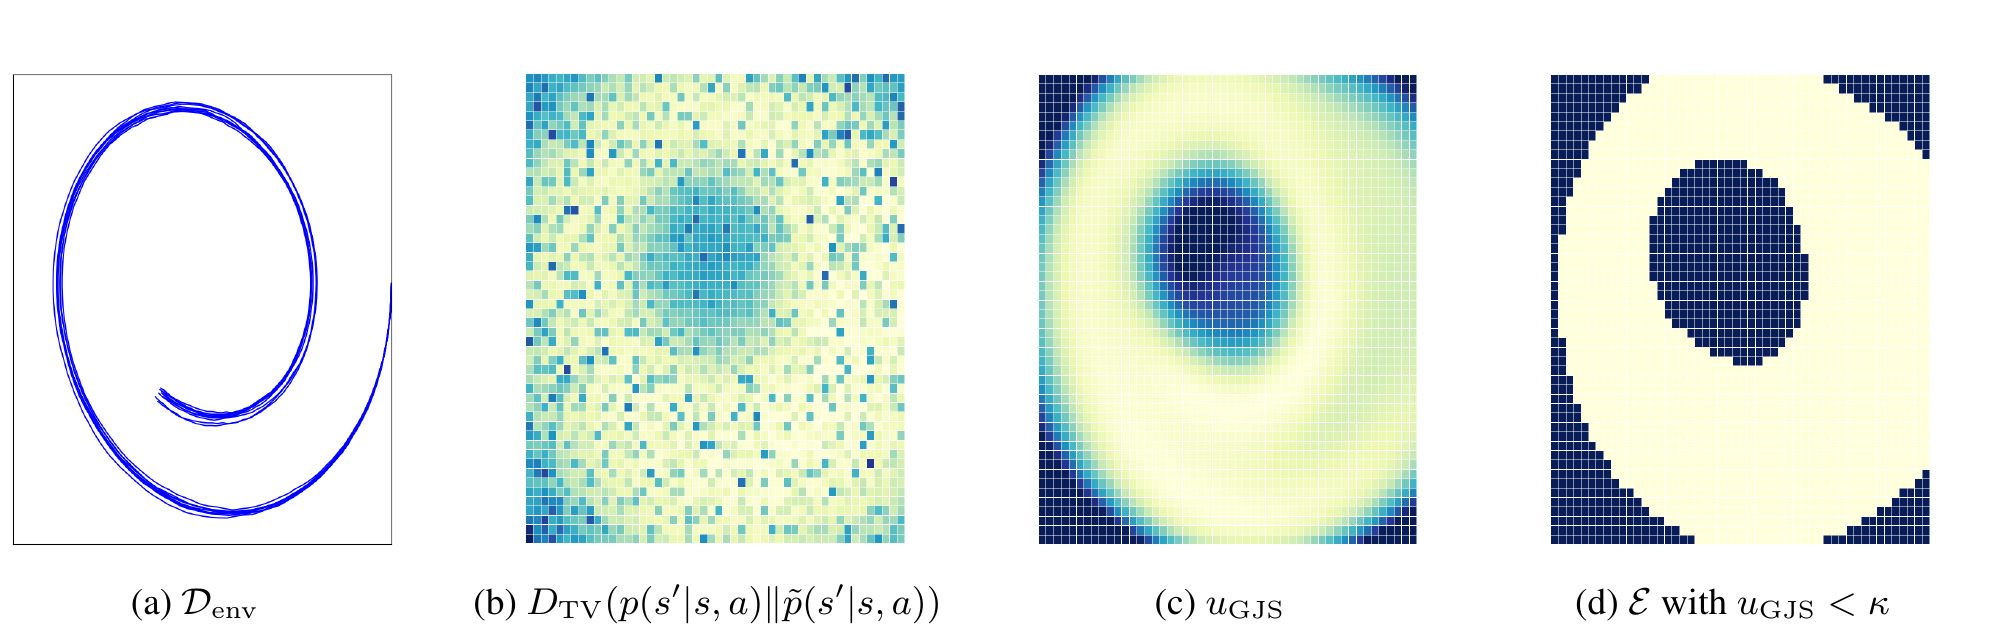
\includegraphics[width=0.54\linewidth]{figures/paper/fig3_toy.png}
    \caption{Pendulum (paper, Fig.~3): (a) the data, (b) the true model error, (c) $\ugjs$, (d) the set $\E$.
             $\ugjs$ is low exactly where the real error is low.}
  \end{figure}
\end{frame}

% ── I.7 ───────────────────────────────────────────────────────────────────────────────────────────
\begin{frame}{Why a New Measure? GJS (MACURA) vs OvR (M2AC)}
  \begin{columns}[T]
    \begin{column}{0.52\textwidth}
      \begin{figure}
        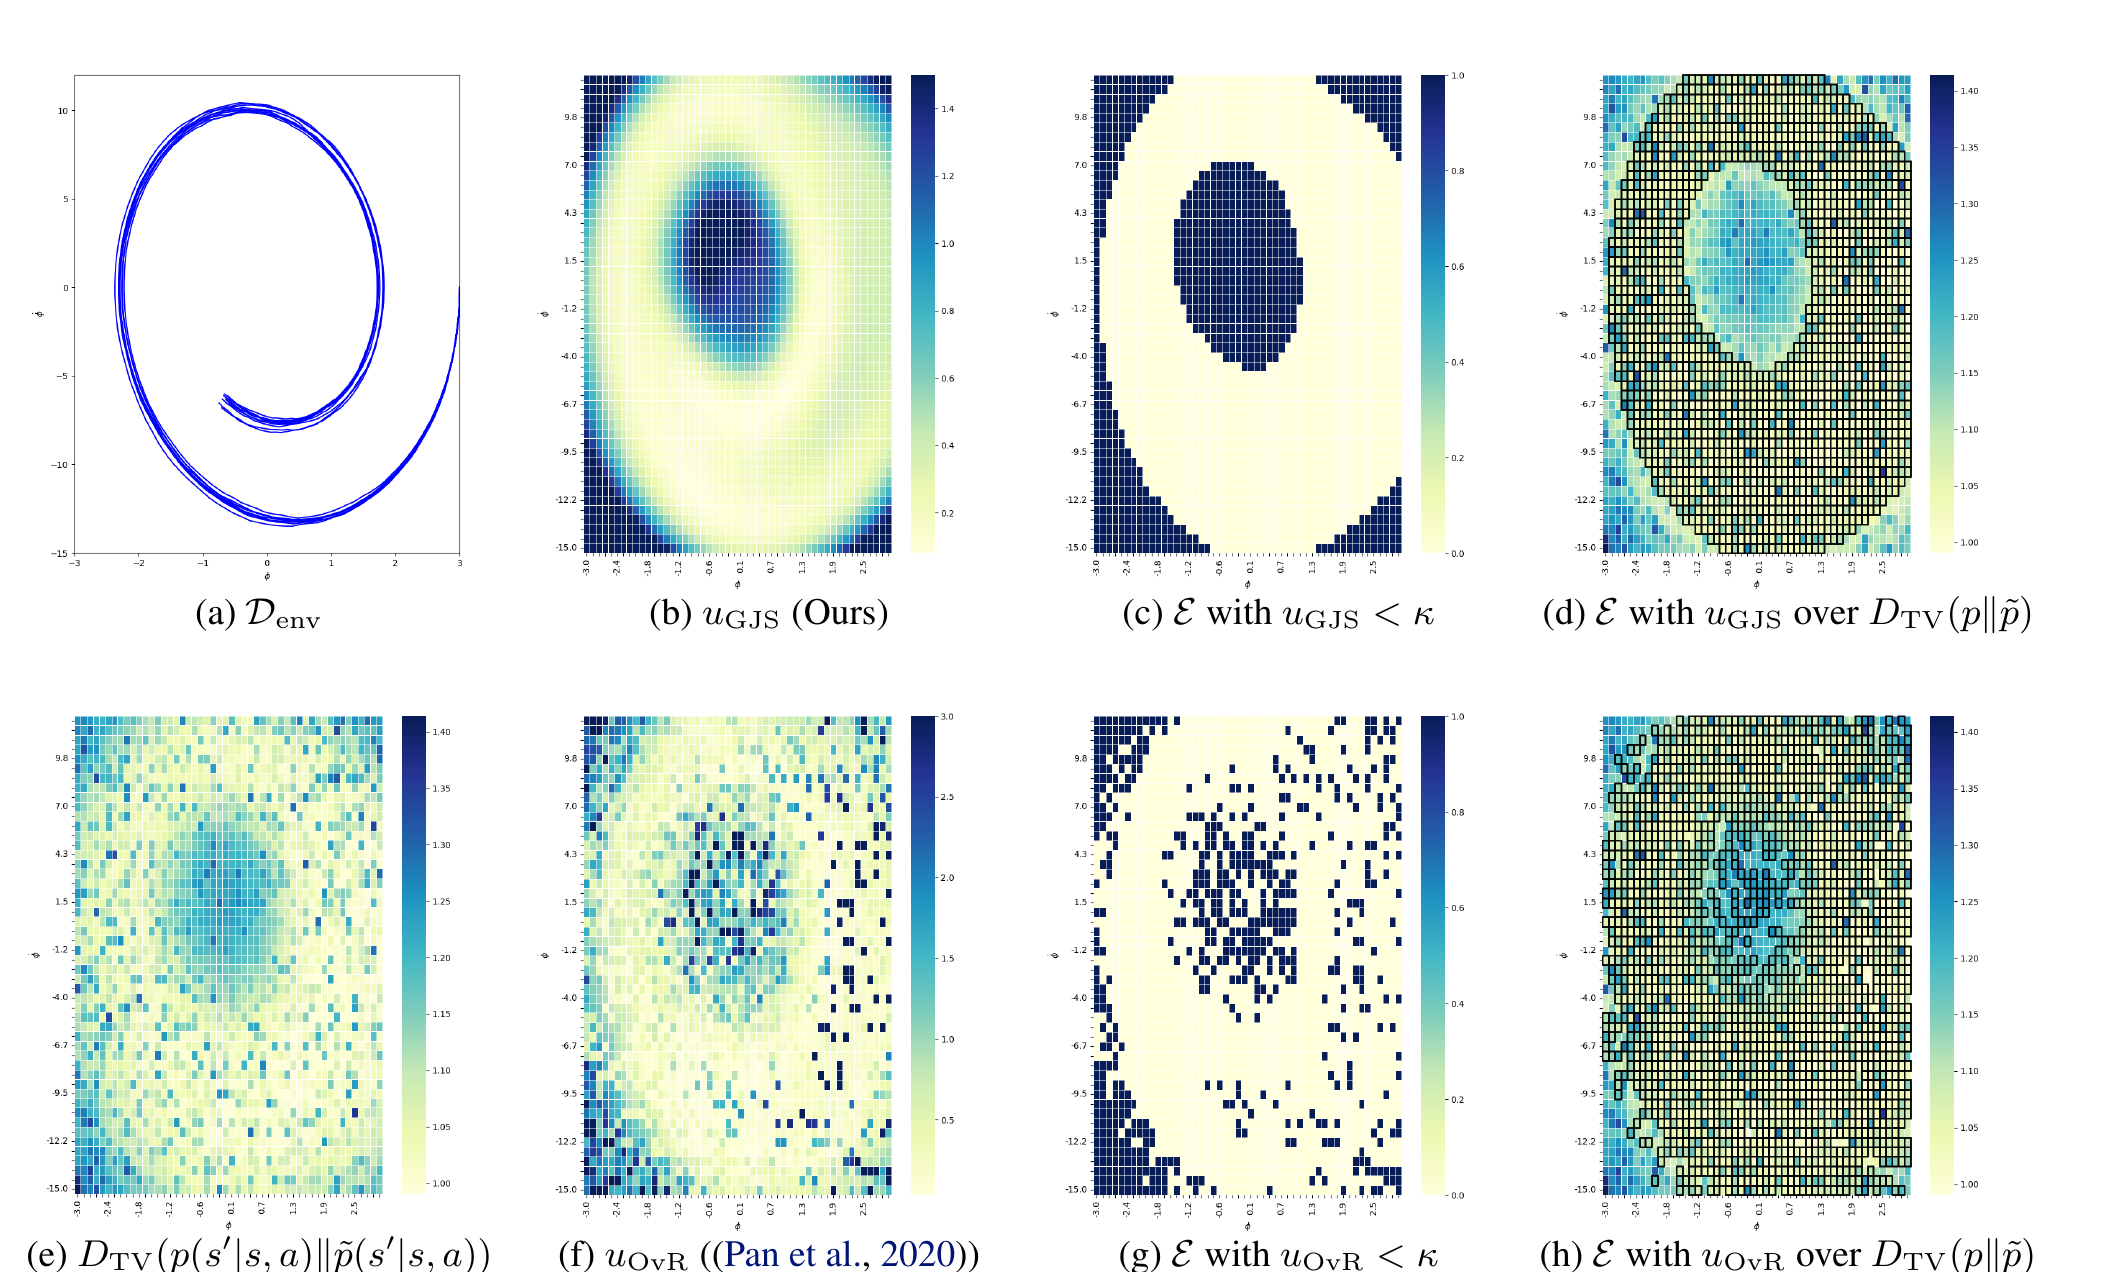
\includegraphics[width=\linewidth]{figures/paper/fig10_gjs_ovr.png}
        \caption{Top: GJS. Bottom: OvR. On the pendulum data (paper, Fig.~10).}
      \end{figure}
    \end{column}
    \begin{column}{0.46\textwidth}
      \small
      \begin{itemize}
        \item \textbf{GJS} (b) is smooth and follows the data. Its set $\E$ (c) has a clear border and matches the
              region of \textbf{low real error} (d).
        \item \textbf{OvR} (f) is \textbf{noisy} and \textbf{over-confident}: it is low in the centre, where the real
              error is high (e). Its set (g) misses the accurate region (h).
        \item The reason: OvR compares \textbf{one} network with the rest; GJS averages \textbf{all pairs}, so one
              lucky network cannot hide the disagreement.
      \end{itemize}
      \vspace{0.3em}
      $\Rightarrow$ To decide \textbf{where} to stop, the uncertainty must be \textbf{reliable}.
    \end{column}
  \end{columns}
\end{frame}

% ── I.8 ───────────────────────────────────────────────────────────────────────────────────────────
\begin{frame}{MACURA: Stop Imagining Where the Model Is Unsure}
  \begin{columns}[T]
    \begin{column}{0.49\textwidth}
      \textbf{1. The stop rule}
      \begin{itemize}\small
        \item At every imagined step, compute $\ugjs(s,a)$.
        \item If $\ugjs<\kappa$: keep the step and continue.
        \item If $\ugjs\ge\kappa$: \textbf{stop the trip}; this step is not kept.
        \item So the trip length becomes \textbf{local}: long where the networks agree, zero where they do not
              (at most $T_{\max}=10$ steps).
      \end{itemize}
      \textbf{2. A threshold that tunes itself}
      \begin{itemize}\small
        \item Each round, take the 95\% quantile ($\zeta$) of the \textbf{first-step} uncertainties: the first step
              starts from a real state, so it shows what ``certain'' looks like now.
        \item $\kappa=\frac{\xi}{K}\sum_{k=1}^{K}\hat u_k$: the average over all rounds, scaled by $\xi$.
      \end{itemize}
    \end{column}
    \begin{column}{0.47\textwidth}
      \textbf{3. Updates that follow the trusted data}
      \[ G=\Big\lfloor G_{\max}\,\tfrac{|\Dmod|}{|\Dmod|_{\max}}\Big\rceil \]
      \begin{itemize}\small
        \item Short trips (a poor model): few SAC updates.
        \item Long trips (a good model): more updates.
      \end{itemize}
      \textbf{4. Exploration with pink noise}
      \begin{itemize}\small
        \item Noise that is correlated in time collects new data at the border of $\E$, so $\E$ grows.
      \end{itemize}
      \vspace{0.3em}
      \colorbox{myblue!10}{\parbox{0.95\linewidth}{\small $T_{\max}=10$ and $\zeta=95\%$ are fixed for every task:
      only $\xi$ is tuned.}}
    \end{column}
  \end{columns}
\end{frame}

% ── I.9 ───────────────────────────────────────────────────────────────────────────────────────────
\begin{frame}{MACURA Architecture}
  \centering
  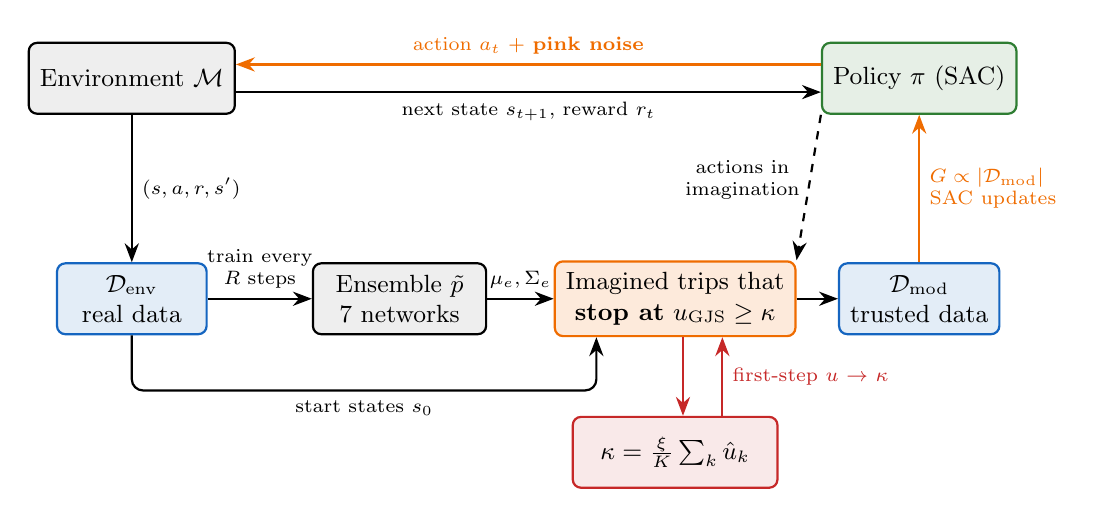
\begin{tikzpicture}
    \node[box, minimum width=2.4cm] (env) at (0,2.8) {Environment $\mathcal{M}$};
    \node[greenbox, minimum width=2.4cm] (pi) at (10.0,2.8) {Policy $\pi$ (SAC)};
    \node[bluebox, minimum width=1.9cm] (denv) at (0,0) {$\Denv$\\real data};
    \node[box, minimum width=2.2cm] (model) at (3.4,0) {Ensemble $\ptil$\\7 networks};
    \node[orangebox, minimum width=2.6cm] (roll) at (6.9,0) {Imagined trips that\\\textbf{stop at} $\ugjs\ge\kappa$};
    \node[bluebox, minimum width=1.9cm] (dmod) at (10.0,0) {$\Dmod$\\trusted data};
    \node[redbox, minimum width=2.6cm] (kappa) at (6.9,-1.95) {$\kappa=\frac{\xi}{K}\sum_k\hat u_{k}$};
    \draw[arr, myorange] ([yshift=5pt]pi.west) -- node[lab, above] {action $a_t$ + \textbf{pink noise}} ([yshift=5pt]env.east);
    \draw[arr] ([yshift=-5pt]env.east) -- node[lab, below] {next state $s_{t+1}$, reward $r_t$} ([yshift=-5pt]pi.west);
    \draw[arr] (env) -- node[lab, right] {$(s,a,r,s')$} (denv);
    \draw[arr] (denv) -- node[lab, above] {train every\\$R$ steps} (model);
    \draw[arr] (model) -- node[lab, above] {$\mu_e,\Sigma_e$} (roll);
    \draw[arr] (roll) -- (dmod);
    \draw[arr, rounded corners] (denv.south) -- ++(0,-0.7) -| node[lab, below, pos=0.25] {start states $s_0$} ([xshift=-1.0cm]roll.south);
    \draw[arr, myred] ([xshift=0.1cm]roll.south) -- ([xshift=0.1cm]kappa.north);
    \draw[arr, myred] ([xshift=0.6cm]kappa.north) -- node[lab, right, text=myred] {first-step $u$ $\to$ $\kappa$} ([xshift=0.6cm]roll.south);
    \draw[arr, myorange] (dmod) -- node[lab, right, align=left, text=myorange] {$G\propto|\Dmod|$\\SAC updates} (pi);
    \draw[arr, dashed] (pi.south west) -- node[lab, left, pos=0.45] {actions in\\imagination} (roll.north east);
  \end{tikzpicture}

  \footnotesize The loop is the same as MBPO's. What MACURA adds is in \textcolor{myorange}{\textbf{orange}} and
  \textcolor{myred}{\textbf{red}}: trips stop where the model is uncertain, $\kappa$ tunes itself, the number of
  updates $G$ adapts, and the agent explores with pink noise.
\end{frame}

\section{I \textperiodcentered{} Comparison}

% ── I.10 ──────────────────────────────────────────────────────────────────────────────────────────
\begin{frame}{How Each Method Handles Its Imagined Trips}
  \small All three start trips from real states, take a random network for each step, and train SAC on the result.
  \textcolor{myorange}{\textbf{Orange}}: where they differ.
  \vspace{0.3em}

  \begin{columns}[T]
    \begin{column}{0.31\textwidth}
      \textbf{MBPO}\\[0.2em]
      \scriptsize
      \begin{algorithmic}
        \State \chg{$k\gets$ schedule(step)}
        \For{\chg{$t=0,\dots,k-1$}}
          \State $a\sim\pi(s)$;\ $s'\sim\ptil_e(s,a)$
          \State \chg{store $(s,a,r,s')$} \Comment{always}
          \State $s\gets s'$
        \EndFor
        \State \chg{$G\gets$ fixed}
      \end{algorithmic}
      \code{mbpo.py: mbpo\_rollout()}
    \end{column}
    \begin{column}{0.33\textwidth}
      \textbf{M2AC}\\[0.2em]
      \scriptsize
      \begin{algorithmic}
        \For{$h=0,\dots,H-1$} \Comment{all trips}
          \State $a\sim\pi(s)$;\ $s'\sim\ptil_e(s,a)$
          \State \chg{$u\gets$ OvR (net $e$ vs rest)}
          \State \chg{keep the $\frac{H-h}{2(H+1)}$ lowest $u$}
          \State \chg{store $(s,a,r-\alpha u,s')$} if kept
          \State $s\gets s'$ \Comment{nobody stops}
        \EndFor
        \State \chg{$G\gets$ fixed}
      \end{algorithmic}
      \code{m2ac.py: m2ac\_rollout()}
    \end{column}
    \begin{column}{0.33\textwidth}
      \textbf{MACURA} (paper, Alg.~2)\\[0.2em]
      \scriptsize
      \begin{algorithmic}
        \For{$t=0,\dots,T_{\max}-1$}
          \State $a\sim\pi(s)$;\ $s'\sim\ptil_e(s,a)$
          \State \chg{$u\gets\ugjs(s,a)$} \Comment{all pairs}
          \State \chg{\textbf{if} $t=0$: update $\kappa$}
          \If{\chg{$u<\kappa$}}
            \State store $(s,a,r,s')$;\ $s\gets s'$
          \Else
            \State \chg{\textbf{stop} this trip}
          \EndIf
        \EndFor
        \State \chg{$G\gets G_{\max}|\Dmod|/|\Dmod|_{\max}$}
      \end{algorithmic}
      \code{macura.py: macura\_rollout()}
    \end{column}
  \end{columns}
  \vspace{0.5em}
  \begin{columns}[T]
    \begin{column}{0.31\textwidth}
      \footnotesize\textcolor{myred}{\textbf{Problem}}: wrong steps are used as if they were right.
    \end{column}
    \begin{column}{0.33\textwidth}
      \footnotesize\textcolor{myred}{\textbf{Problem}}: a fixed share, whatever the quality; a noisy measure.
    \end{column}
    \begin{column}{0.33\textwidth}
      \footnotesize\textcolor{mygreen}{\textbf{Strength}}: keeps exactly the steps the networks agree on.
    \end{column}
  \end{columns}
\end{frame}

% ── I.11 ──────────────────────────────────────────────────────────────────────────────────────────
\begin{frame}{Which Imagined Data Are Kept?}
  \centering
  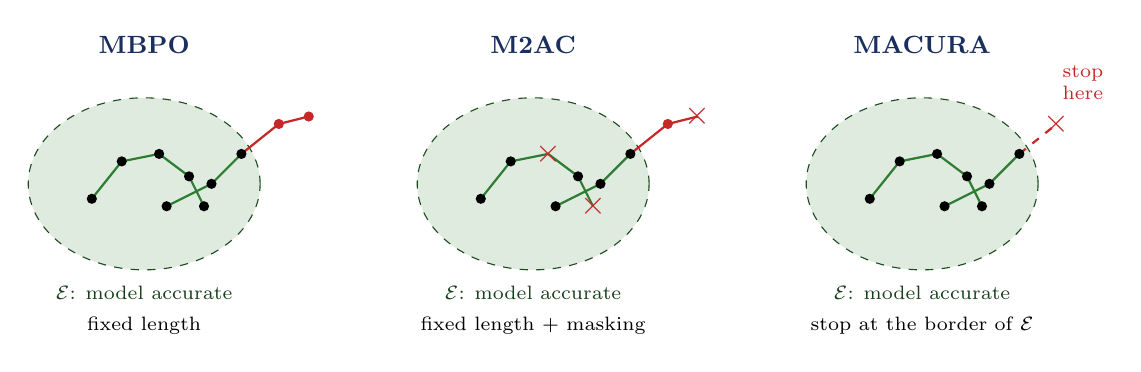
\begin{tikzpicture}[scale=0.95,
      pt/.style={circle, fill=black, inner sep=1.3pt},
      good/.style={thick, mygreen},
      bad/.style={thick, myred},
      cut/.style={myred, very thick}]
    \foreach \x/\name/\sub in {0/MBPO/fixed length, 5.2/M2AC/fixed length + masking, 10.4/MACURA/stop at the border of $\mathcal{E}$} {
      \begin{scope}[xshift=\x cm]
        \fill[mygreen!15] (2,1.5) ellipse (1.55cm and 1.15cm);
        \draw[mygreen!60!black, dashed] (2,1.5) ellipse (1.55cm and 1.15cm);
        \node[font=\scriptsize, text=mygreen!50!black] at (2,0.05) {$\mathcal{E}$: model accurate};
        \node[font=\small\bfseries, text=navy] at (2,3.35) {\name};
        \node[font=\scriptsize] at (2,-0.4) {\sub};
      \end{scope}
    }
    \begin{scope}
      \draw[good] (1.3,1.3) -- (1.7,1.8) -- (2.2,1.9) -- (2.6,1.6) -- (2.8,1.2);
      \draw[good] (2.3,1.2) -- (2.9,1.5) -- (3.3,1.9);
      \draw[bad]  (3.3,1.9) -- (3.8,2.3) -- (4.2,2.4);
      \foreach \p in {(1.3,1.3),(1.7,1.8),(2.2,1.9),(2.6,1.6),(2.8,1.2),(2.3,1.2),(2.9,1.5),(3.3,1.9)} \node[pt] at \p {};
      \foreach \p in {(3.8,2.3),(4.2,2.4)} \node[pt, fill=myred] at \p {};
    \end{scope}
    \begin{scope}[xshift=5.2cm]
      \draw[good] (1.3,1.3) -- (1.7,1.8) -- (2.2,1.9) -- (2.6,1.6) -- (2.8,1.2);
      \draw[good] (2.3,1.2) -- (2.9,1.5) -- (3.3,1.9);
      \draw[bad]  (3.3,1.9) -- (3.8,2.3) -- (4.2,2.4);
      \foreach \p in {(1.3,1.3),(1.7,1.8),(2.6,1.6),(2.3,1.2),(2.9,1.5),(3.3,1.9)} \node[pt] at \p {};
      \node[pt, fill=myred] at (3.8,2.3) {};
      \foreach \p in {(2.2,1.9),(2.8,1.2),(4.2,2.4)} \node[cut] at \p {\large$\times$};
    \end{scope}
    \begin{scope}[xshift=10.4cm]
      \draw[good] (1.3,1.3) -- (1.7,1.8) -- (2.2,1.9) -- (2.6,1.6) -- (2.8,1.2);
      \draw[good] (2.3,1.2) -- (2.9,1.5) -- (3.3,1.9);
      \draw[bad, dashed] (3.3,1.9) -- (3.8,2.3);
      \foreach \p in {(1.3,1.3),(1.7,1.8),(2.2,1.9),(2.6,1.6),(2.8,1.2),(2.3,1.2),(2.9,1.5),(3.3,1.9)} \node[pt] at \p {};
      \node[cut] at (3.8,2.3) {\large$\times$};
      \node[font=\scriptsize, text=myred, align=center] at (4.15,2.85) {stop\\here};
    \end{scope}
  \end{tikzpicture}
  \vspace{0.5em}
  \begin{itemize}\small
    \item \textbf{MBPO}: every trip has the same length, so the imagined steps \textbf{outside} $\E$ (\textcolor{myred}{red})
          are used for training.
    \item \textbf{M2AC}: the same trips, then a \textbf{fixed share} of uncertain steps is removed ($\times$), wherever
          they are, even inside $\E$.
    \item \textbf{MACURA}: each trip \textbf{stops at its first uncertain step}: long inside $\E$, nothing outside.
  \end{itemize}
\end{frame}

% ── I.12 ──────────────────────────────────────────────────────────────────────────────────────────
\begin{frame}{The Four Algorithms Side by Side}
  \centering
  \footnotesize
  \renewcommand{\arraystretch}{1.1}\setlength{\tabcolsep}{4pt}
  \begin{tabular}{>{\raggedright\arraybackslash\bfseries}p{2.3cm}*{3}{>{\raggedright\arraybackslash}p{2.35cm}}>{\raggedright\arraybackslash}p{3.2cm}}
    \toprule
    & \textbf{SAC} & \textbf{MBPO} & \textbf{M2AC} & \textbf{MACURA} \\
    \midrule
    world model & none & 7-network ensemble & same & same \\
    question it answers & -- & \emph{when} to trust & \emph{how much} to trust & \emph{where} to trust \\
    trip length & -- & fixed $k$, by schedule & fixed horizon $H$ & \textbf{adaptive}, until $\ugjs\ge\kappa$ \\
    imagined data used & -- & all of it & a fixed share ($\approx$25\%) & only steps \textbf{inside} $\E$ \\
    uncertainty & -- & none & OvR (one vs rest) & GJS (all pairs) \\
    stored reward & $r$ & $r$ & $r-\alpha u$ & $r$ \\
    SAC updates per step & 1 & fixed $G$ & fixed $G$ & \textbf{adaptive} $G\propto|\Dmod|$ \\
    exploration (paper) & samples its policy & deterministic & deterministic & \textbf{pink noise} \\
    tuned per task & -- & the schedule & share, penalty $\alpha$ & only $\xi$ \\
    \bottomrule
  \end{tabular}
  \vspace{0.3em}

  \small The three model-based methods share the SAC learner, the ensemble and the 95\%/5\% data mix. They differ
  \textbf{only in which imagined data reach the learner}, and how much it trains on them.
\end{frame}

\section{I \textperiodcentered{} Results}

% ── I.13 ──────────────────────────────────────────────────────────────────────────────────────────
\begin{frame}{How Far Each Method Imagines, and How Much It Trains}
  \begin{columns}[T]
    \begin{column}{0.49\textwidth}
      \begin{figure}
        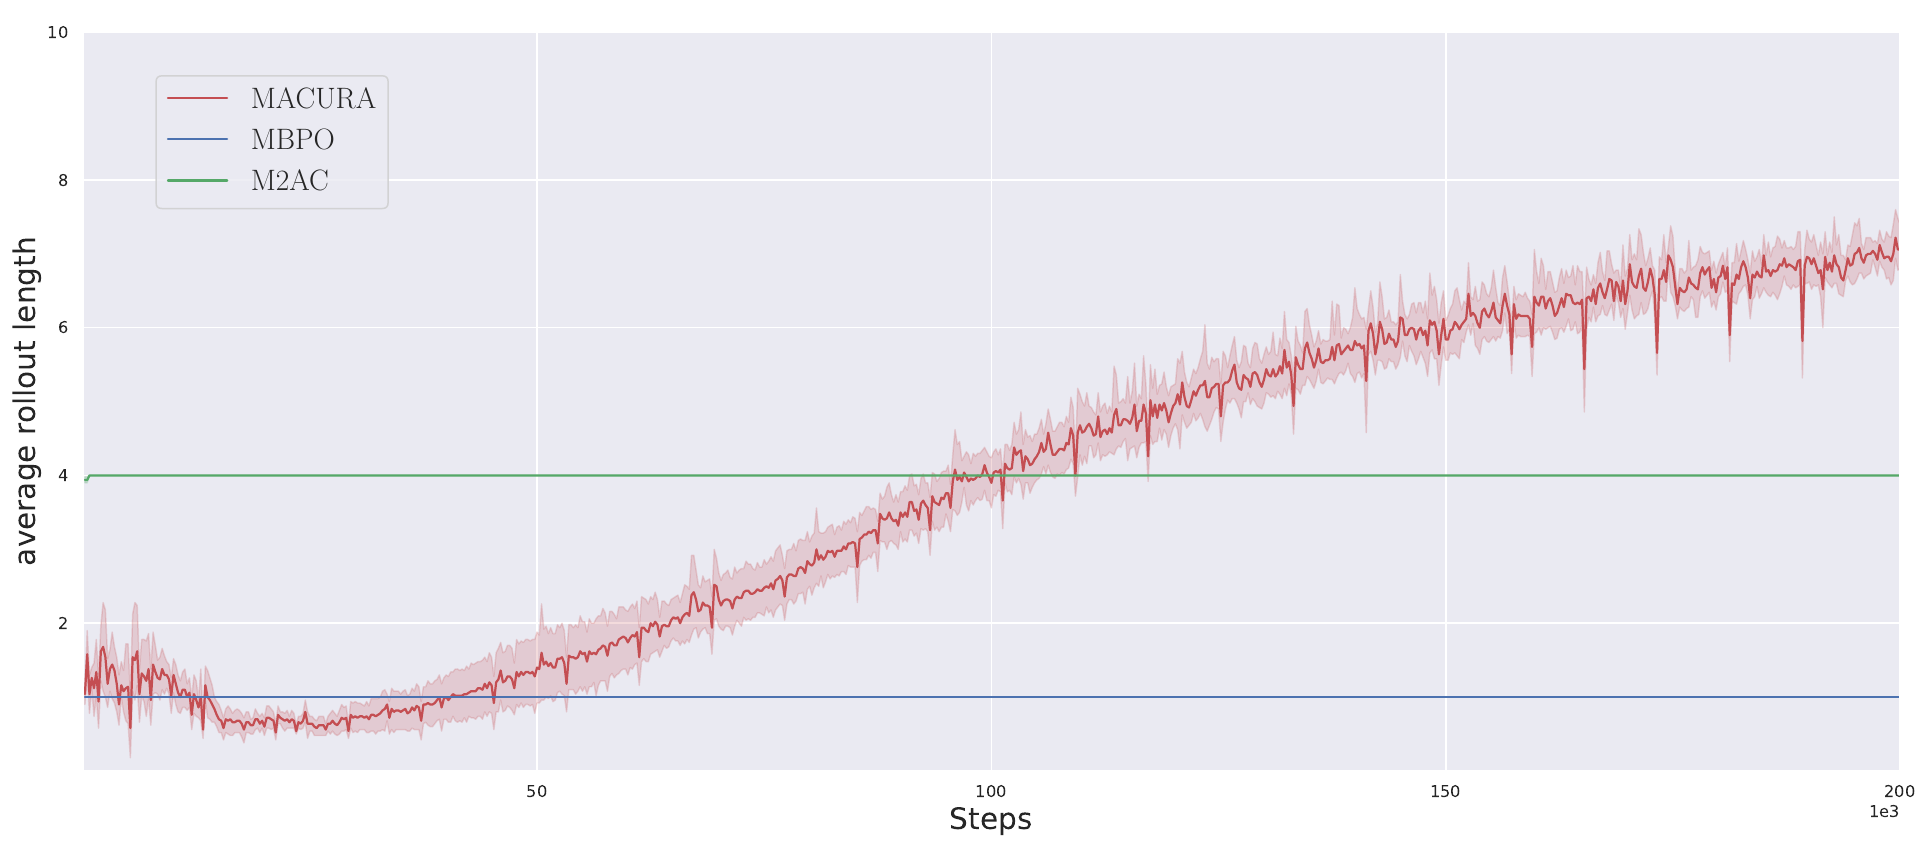
\includegraphics[width=0.86\linewidth]{figures/paper/fig17_rollout_len.png}
        \caption{Average trip length on Walker (paper, Fig.~17).}
      \end{figure}
      \vspace{-0.4em}
      \begin{itemize}\footnotesize
        \item \textbf{MBPO}: length 1 all along (its tuned schedule). \textbf{M2AC}: a constant average.
        \item \textbf{MACURA}: short while the model is poor (even below 1: it can drop the first step), then
              growing to about 7.
      \end{itemize}
    \end{column}
    \begin{column}{0.49\textwidth}
      \begin{figure}
        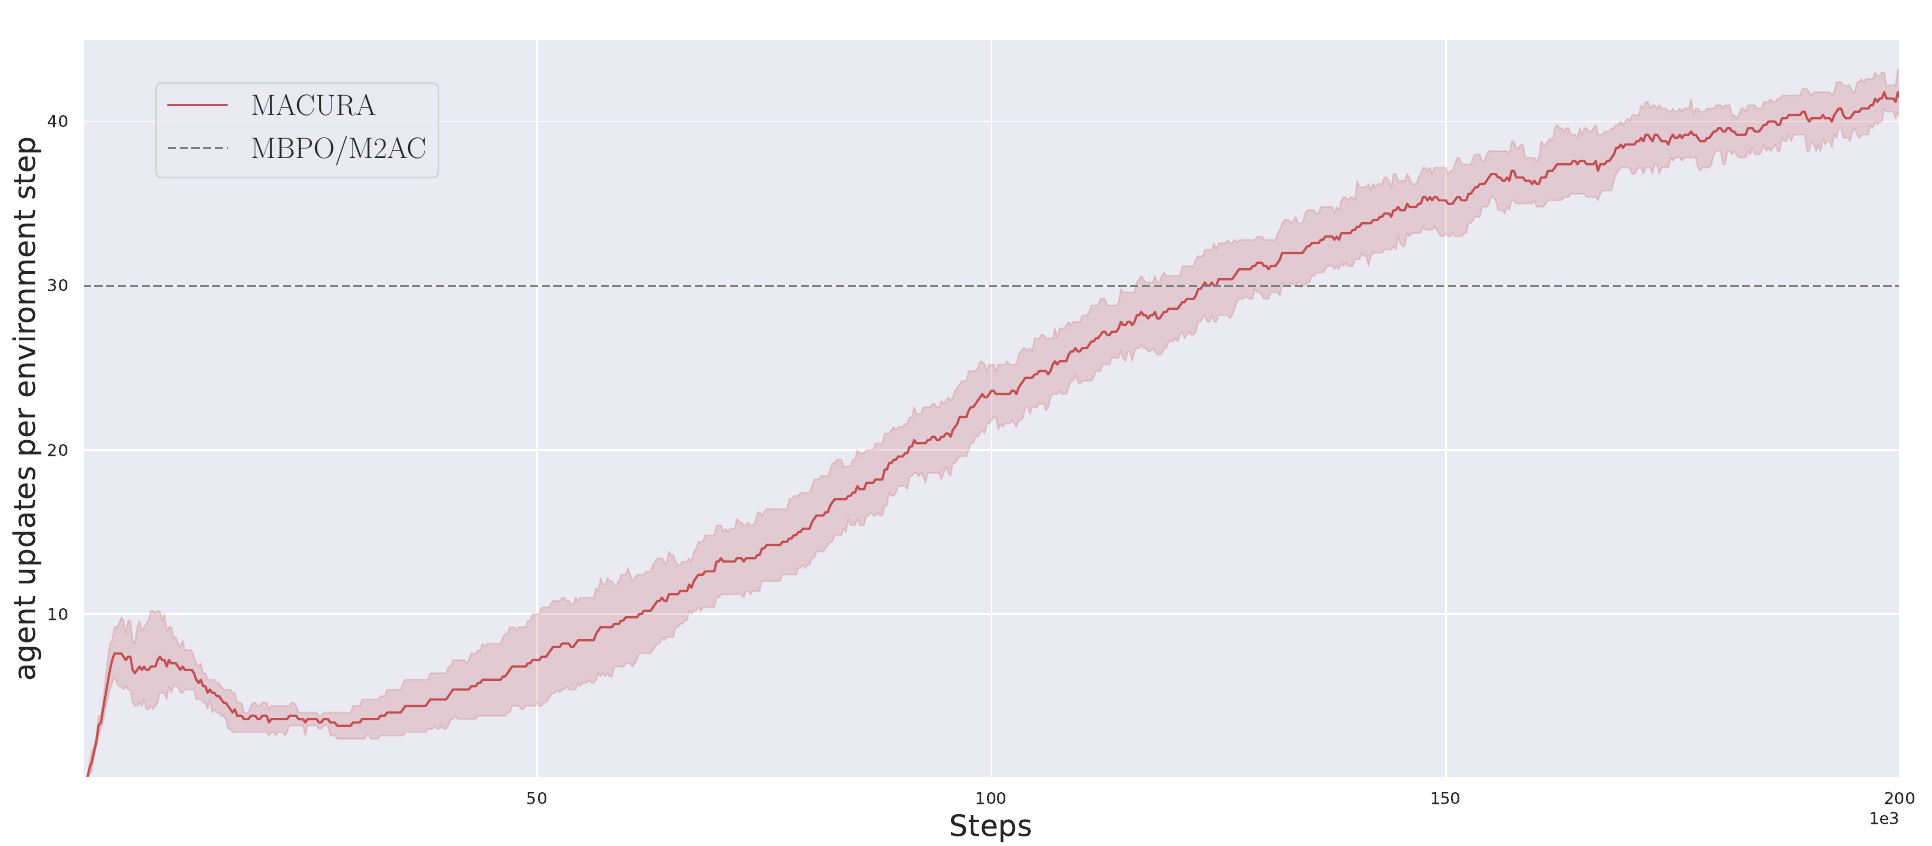
\includegraphics[width=0.86\linewidth]{figures/paper/fig19_updates.png}
        \caption{SAC updates per real step on Walker (paper, Fig.~19).}
      \end{figure}
      \vspace{-0.4em}
      \begin{itemize}\footnotesize
        \item MACURA's updates \textbf{follow its trusted data}: few at first, then more than the fixed 30 of MBPO
              and M2AC.
        \item More updates alone do not explain it: with 40 updates per step, MBPO and M2AC still stay behind.
      \end{itemize}
    \end{column}
  \end{columns}
\end{frame}

% ── I.14 ──────────────────────────────────────────────────────────────────────────────────────────
\begin{frame}{Two Kinds of Noise}
  \begin{columns}[T]
    \begin{column}{0.49\textwidth}
      \textbf{1. Exploration noise}: how the agent collects data
      \begin{figure}
        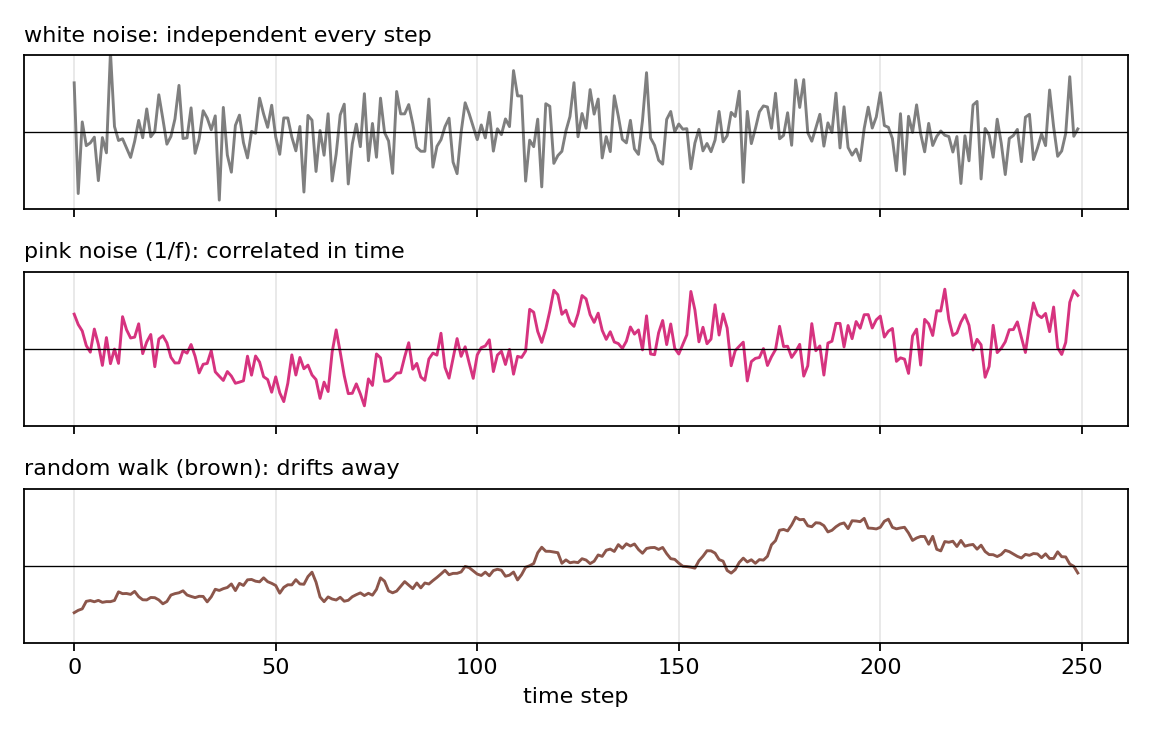
\includegraphics[width=0.8\linewidth]{figures/project/noise_types.png}
      \end{figure}
      \vspace{-0.6em}
      \begin{itemize}\footnotesize
        \item \textbf{White noise} is independent at every step, so its pushes cancel out.
        \item \textbf{Pink noise} ($1/f$) is correlated in time: it pushes the same way for a while and reaches
              \textbf{new states}, without drifting away.
      \end{itemize}
    \end{column}
    \begin{column}{0.49\textwidth}
      \textbf{2. Environment noise}: the world itself is random
      \begin{figure}
        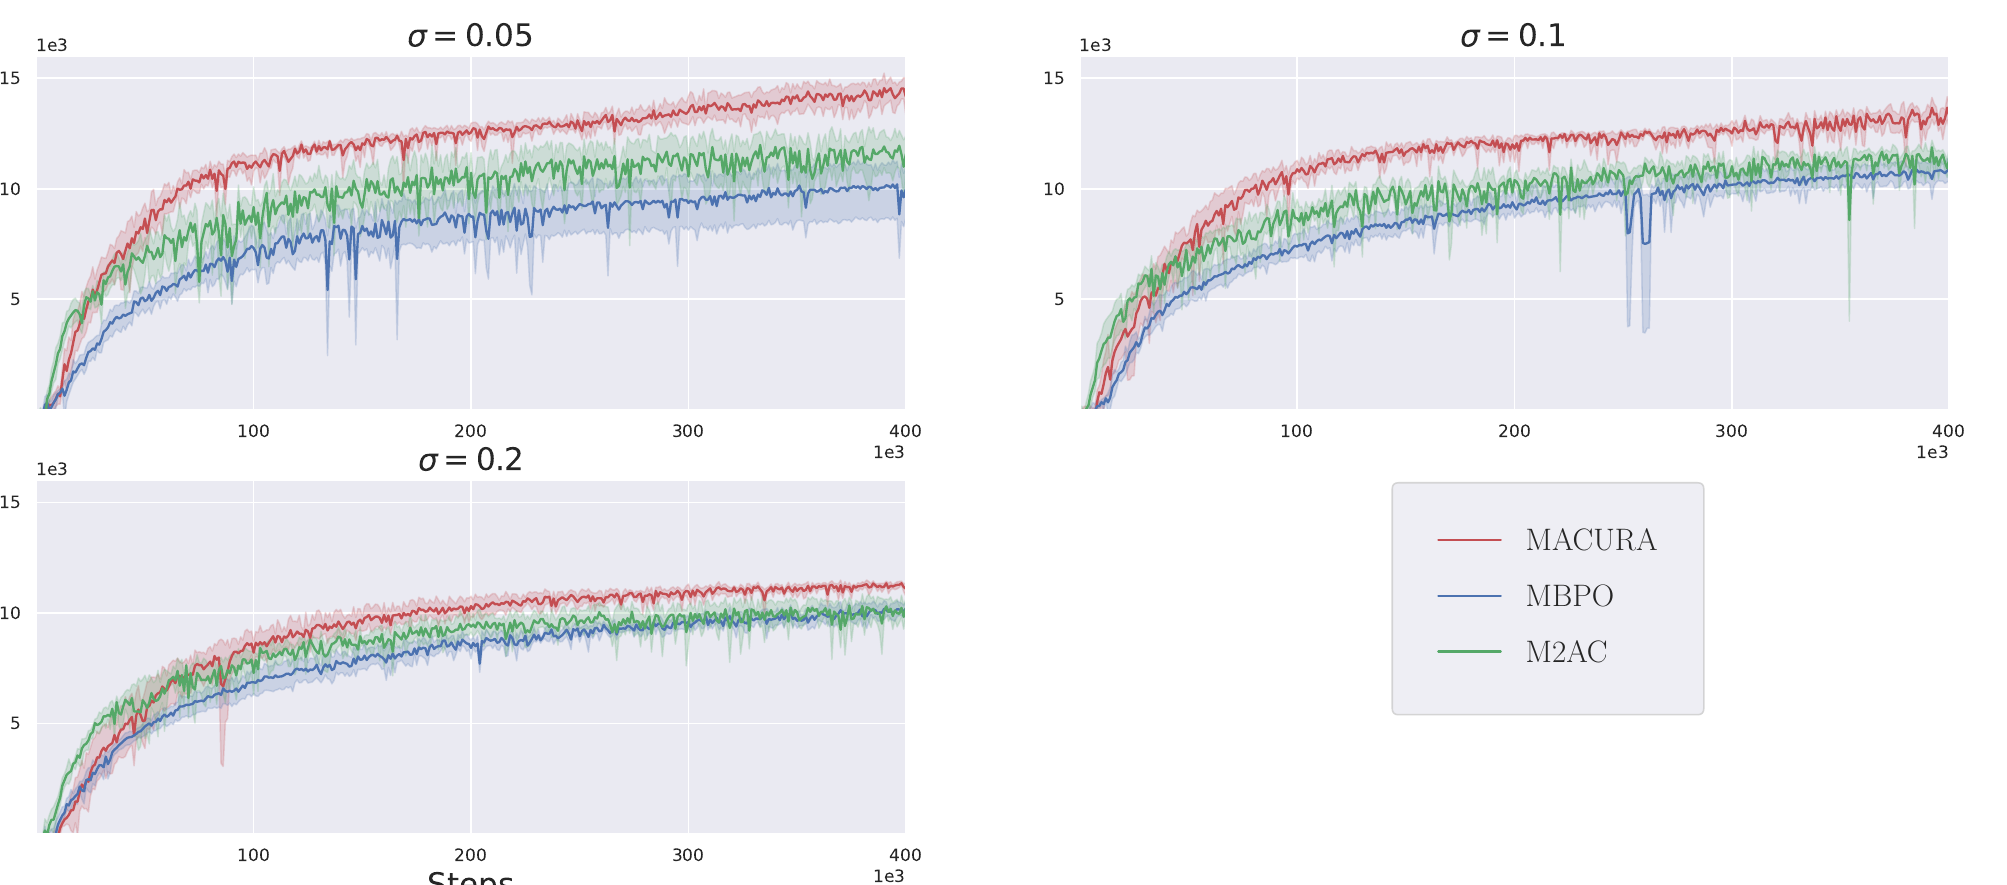
\includegraphics[width=0.8\linewidth]{figures/paper/fig16_noise.png}
        \caption{HalfCheetah with hidden action noise (paper, Fig.~16).}
      \end{figure}
      \vspace{-0.5em}
      \begin{itemize}\footnotesize
        \item The networks learn noise as a \textbf{wide} Gaussian. If they agree, $\ugjs\approx0$ and the step is
              still trusted.
        \item MACURA stops for \textbf{disagreement}, not for noise, and stays ahead at every noise level.
      \end{itemize}
    \end{column}
  \end{columns}
\end{frame}

% ── I.15 ──────────────────────────────────────────────────────────────────────────────────────────
\begin{frame}{Results on MuJoCo}
  \begin{figure}
    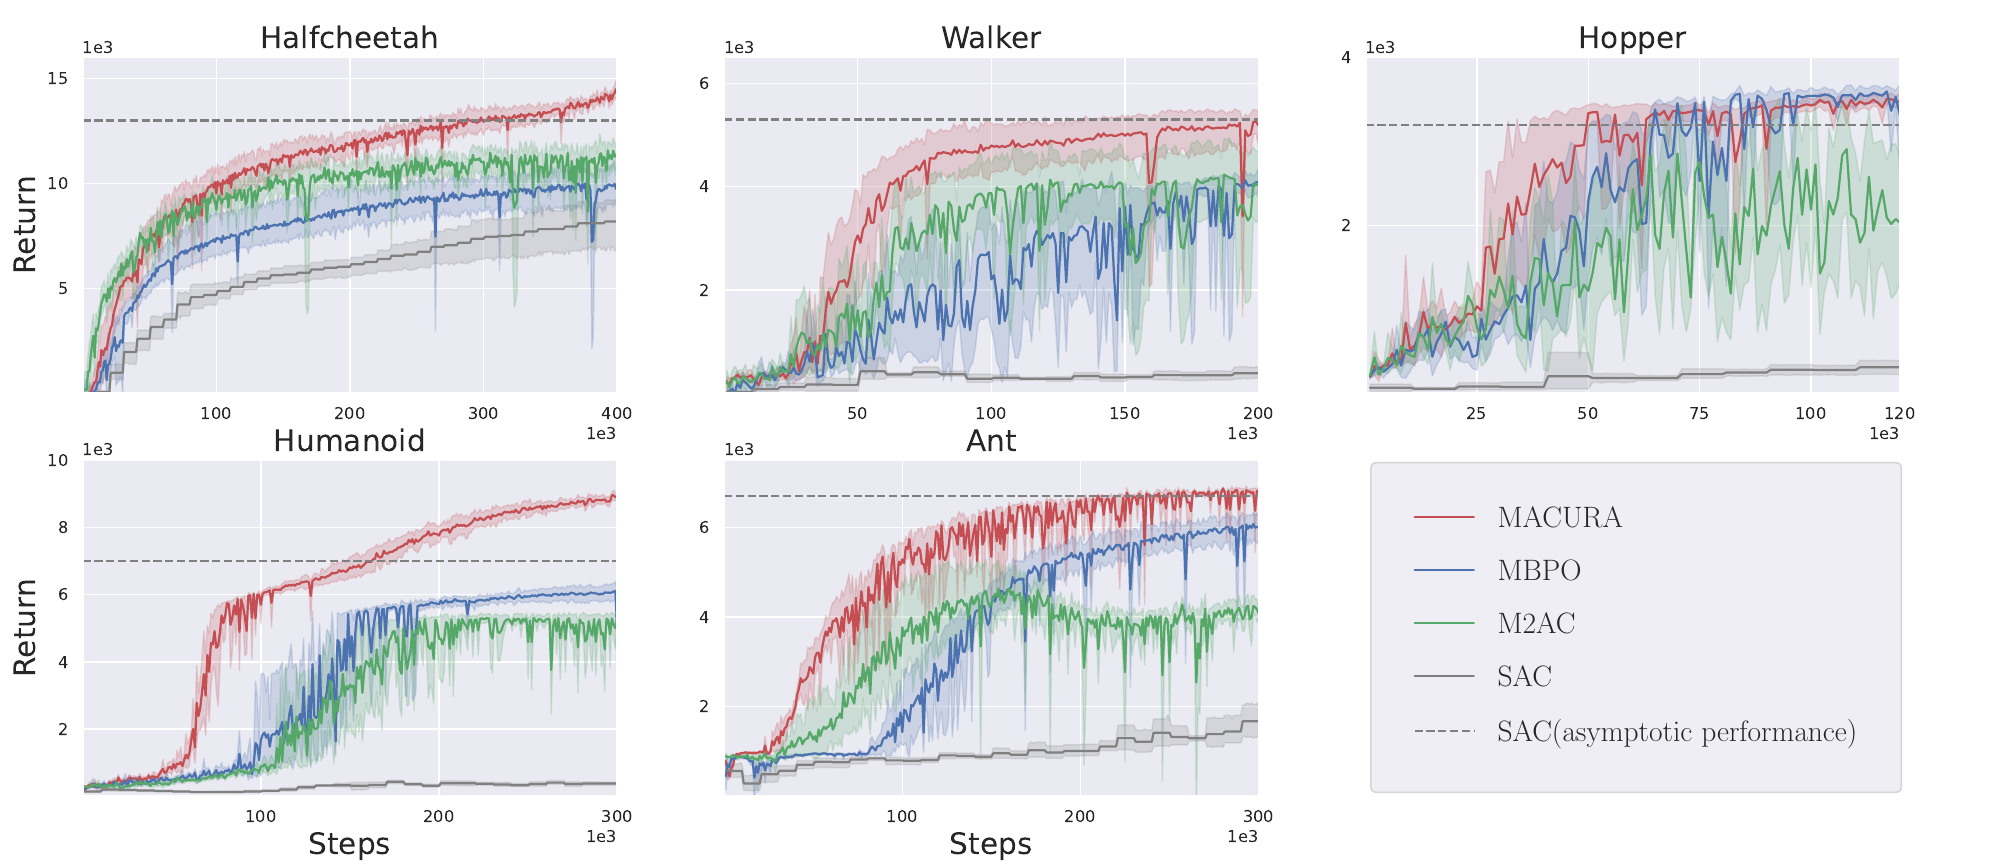
\includegraphics[width=0.63\linewidth]{figures/paper/fig4_mujoco.png}
    \caption{Return while learning on five MuJoCo tasks; mean of 5 seeds with 95\% CI (paper, Fig.~4).}
  \end{figure}
  \vspace{-0.3em}
  \begin{itemize}\small
    \item MACURA learns \textbf{faster} and ends \textbf{higher} than MBPO and M2AC, most clearly on Humanoid and Ant.
    \item It often reaches the final return of model-free SAC with a fraction of the real data.
    \item The reason: long trips where the model is reliable and none where it is not, so the learner gets
          \textbf{more data and cleaner data}.
  \end{itemize}
\end{frame}

% ── I.16 ──────────────────────────────────────────────────────────────────────────────────────────
\begin{frame}{Exploration Changes the Results}
  \begin{columns}[T]
    \begin{column}{0.5\textwidth}
      \begin{figure}
        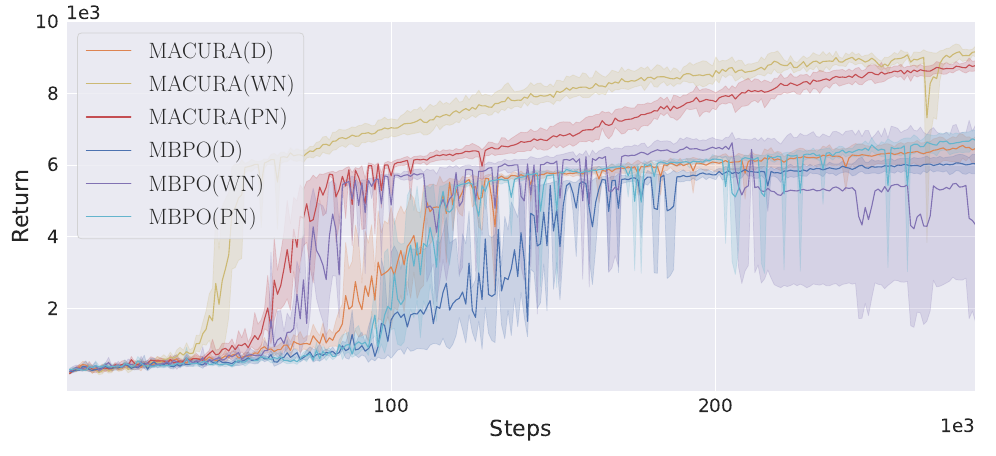
\includegraphics[width=\linewidth]{figures/paper/fig5_exploration.png}
        \caption{Humanoid: deterministic (D), white noise (WN) and pink noise (PN) exploration (paper, Fig.~5).}
      \end{figure}
    \end{column}
    \begin{column}{0.48\textwidth}
      \small
      \begin{itemize}
        \item \textbf{Deterministic}: limited but \textbf{stable}, for both methods.
        \item \textbf{White noise}: can be very strong for MACURA, but it \textbf{destabilises} MBPO.
        \item \textbf{Pink noise}: the best balance of performance and stability.
        \item MACURA gains the most from better exploration: new data grow $\E$, exactly where it uses the model.
        \item With deterministic exploration for \textbf{all} methods, MACURA is still the strongest on most tasks
              (paper appendix).
      \end{itemize}
      \vspace{0.3em}
      \footnotesize Note: the main comparison gives pink noise only to MACURA. I kept this protocol in my project.
    \end{column}
  \end{columns}
\end{frame}

% ── I.17 ──────────────────────────────────────────────────────────────────────────────────────────
\begin{frame}{What Matters? Ablations and the Threshold}
  \begin{columns}[T]
    \begin{column}{0.47\textwidth}
      \begin{figure}
        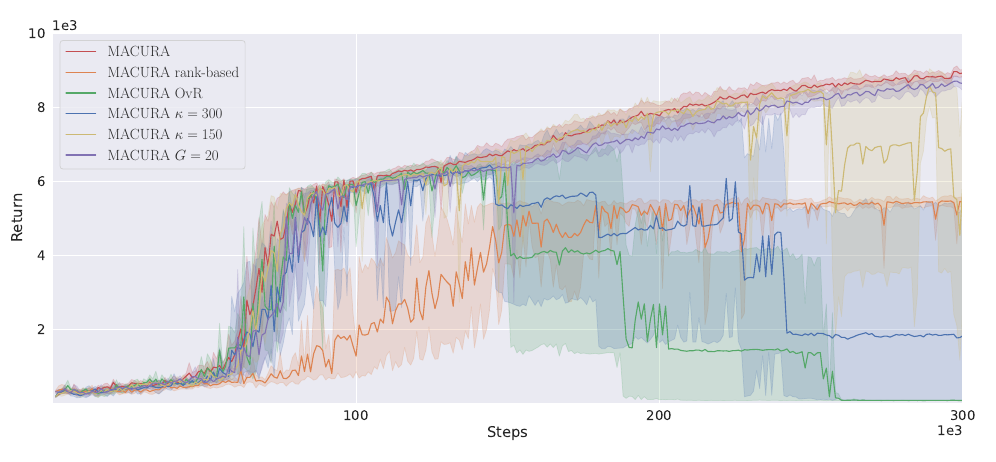
\includegraphics[width=0.85\linewidth]{figures/paper/fig7_ablation.png}
        \caption{Humanoid, one building block changed (paper, Fig.~7).}
      \end{figure}
      \vspace{-0.8em}
      \begin{figure}
        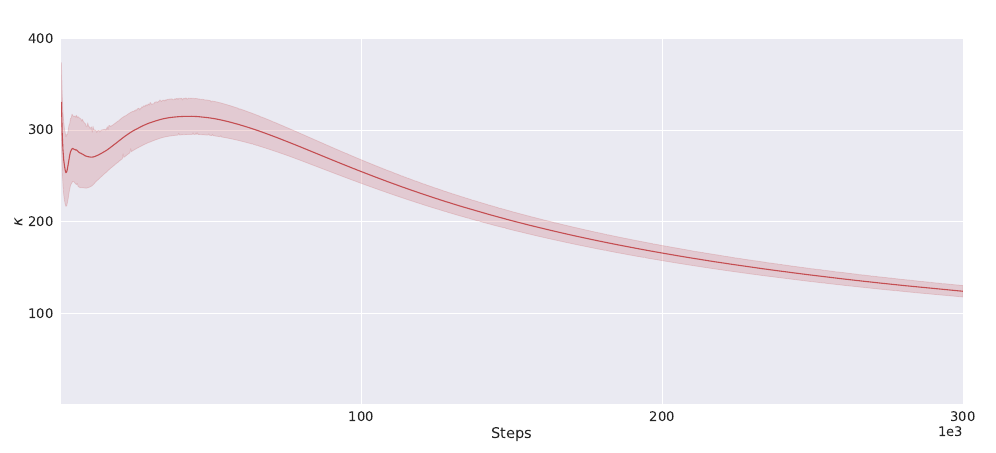
\includegraphics[width=0.42\linewidth]{figures/paper/fig8_kappa.png}
        \caption{$\kappa$ during training (paper, Fig.~8).}
      \end{figure}
    \end{column}
    \begin{column}{0.51\textwidth}
      \small
      \begin{itemize}
        \item M2AC's \textbf{rank rule} instead of a threshold: much worse.
        \item \textbf{OvR} instead of GJS: training \textbf{diverges}, because wrong data get through.
        \item A \textbf{fixed} $\kappa$: unstable at some stage. The adaptive $\kappa$ starts high (rough data are
              enough at first) and then drops (precise data are needed later): a schedule that \textbf{emerges by
              itself}.
        \item A \textbf{fixed} number of updates: a moderate loss.
        \item $\xi$ works over a \textbf{wide range}; too large exploits model errors, too small overfits.
      \end{itemize}
    \end{column}
  \end{columns}
\end{frame}

% ── I.18 ──────────────────────────────────────────────────────────────────────────────────────────
\begin{frame}{The Paper in Short}
  \begin{columns}[T]
    \begin{column}{0.5\textwidth}
      \textbf{Takeaways}
      \begin{itemize}\small
        \item Ask \emph{where}, not \emph{when}, to trust the model.
        \item Imagined trips that stay inside $\E$ guarantee that improvement carries over to reality.
        \item GJS is a cheap, closed-form, reliable measure of \textbf{disagreement}, not of noise.
        \item Trips stop at the first uncertain step; $\kappa$ and $G$ tune themselves.
        \item One knob, $\xi$, and better data efficiency than MBPO and M2AC.
      \end{itemize}
    \end{column}
    \begin{column}{0.46\textwidth}
      \textbf{Limits}
      \begin{itemize}\small
        \item $\xi$ still differs a lot between tasks (0.3 to 30).
        \item Very long training destabilises MBPO and MACURA alike.
        \item The main comparison gives \textbf{pink noise only to MACURA}.
        \item Only simulated locomotion tasks.
      \end{itemize}
    \end{column}
  \end{columns}
  \vspace{1em}
  \centering
  \colorbox{myblue!10}{\parbox{0.9\linewidth}{\centering\small
    \textbf{My question}: does MACURA's advantage hold on a \textbf{new task I built myself}, with the same compute
    for every method, and does it really trust its model less \textbf{where the model is wrong}?}}
\end{frame}

% ════════════════════════════════════════════════════════════════════════════════════════════════
\partslide{II}{My Project: MACURA Races a Drone}{A new task, four algorithms, a fair comparison}
\section{II \textperiodcentered{} Setup}

% ── II.1 ──────────────────────────────────────────────────────────────────────────────────────────
\begin{frame}{The Project: Question and Hypotheses}
  \begin{columns}[T]
    \begin{column}{0.52\textwidth}
      \textbf{Goal}: compare the four algorithms of the paper on a task where I \textbf{know} where a learned model
      will be wrong.
      \begin{itemize}\small
        \item \textbf{Why a drone}: real flights are costly and a crash breaks it, so data efficiency matters.
        \item \textbf{The same for all}: learner, ensemble, data mix, real steps and test scenarios.
              \textbf{Only the rule for imagined trips differs}.
        \item \textbf{MACURA} against \textbf{MBPO} (its base), \textbf{M2AC} (the closest) and \textbf{SAC} (no model).
      \end{itemize}
      \begin{block}{Two hypotheses}
        \small
        \textbf{H1}: with the same compute, MACURA learns faster and scores higher.\\[0.2em]
        \textbf{H2}: MACURA trusts its model \textbf{less where the model is wrong} and trains on fewer wrong
        imagined data.
      \end{block}
    \end{column}
    \begin{column}{0.46\textwidth}
      \begin{figure}
        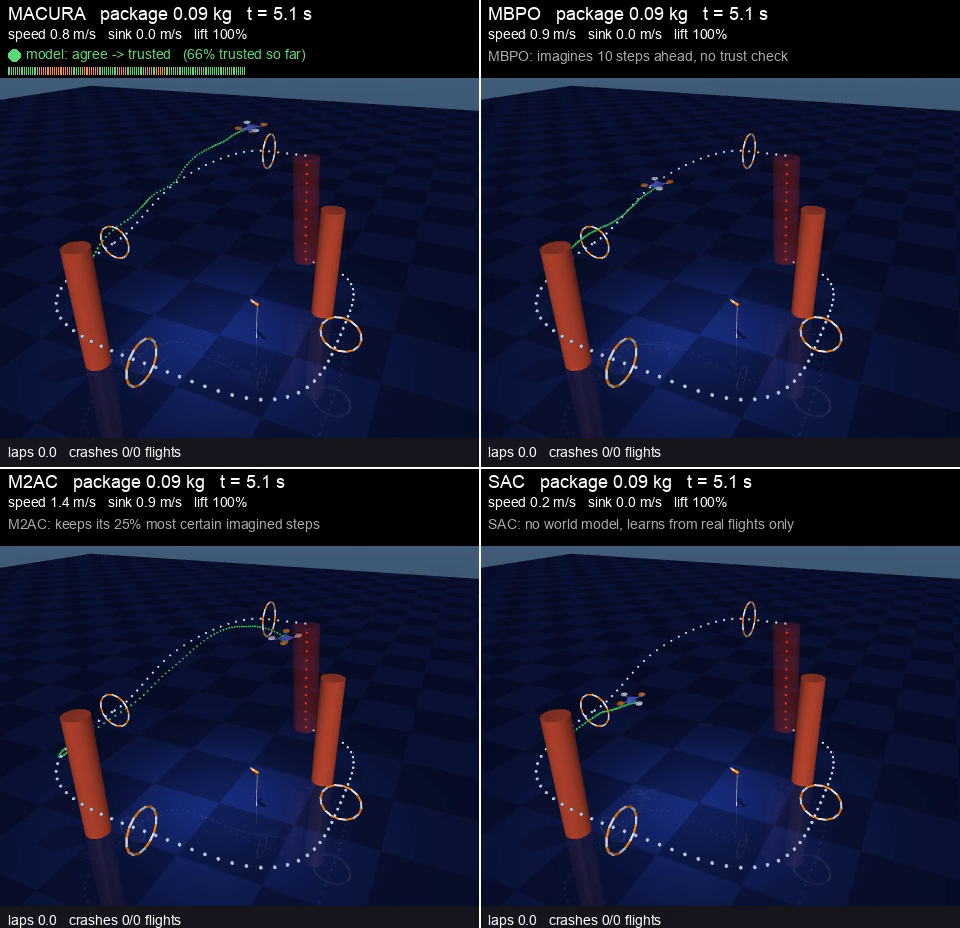
\includegraphics[height=0.58\textheight]{figures/project/frame_all_four.png}
        \caption{The four trained drones on the same new scenario.}
      \end{figure}
    \end{column}
  \end{columns}
\end{frame}

% ── II.2 ──────────────────────────────────────────────────────────────────────────────────────────
\begin{frame}{The Task: Race3}
  \begin{figure}
    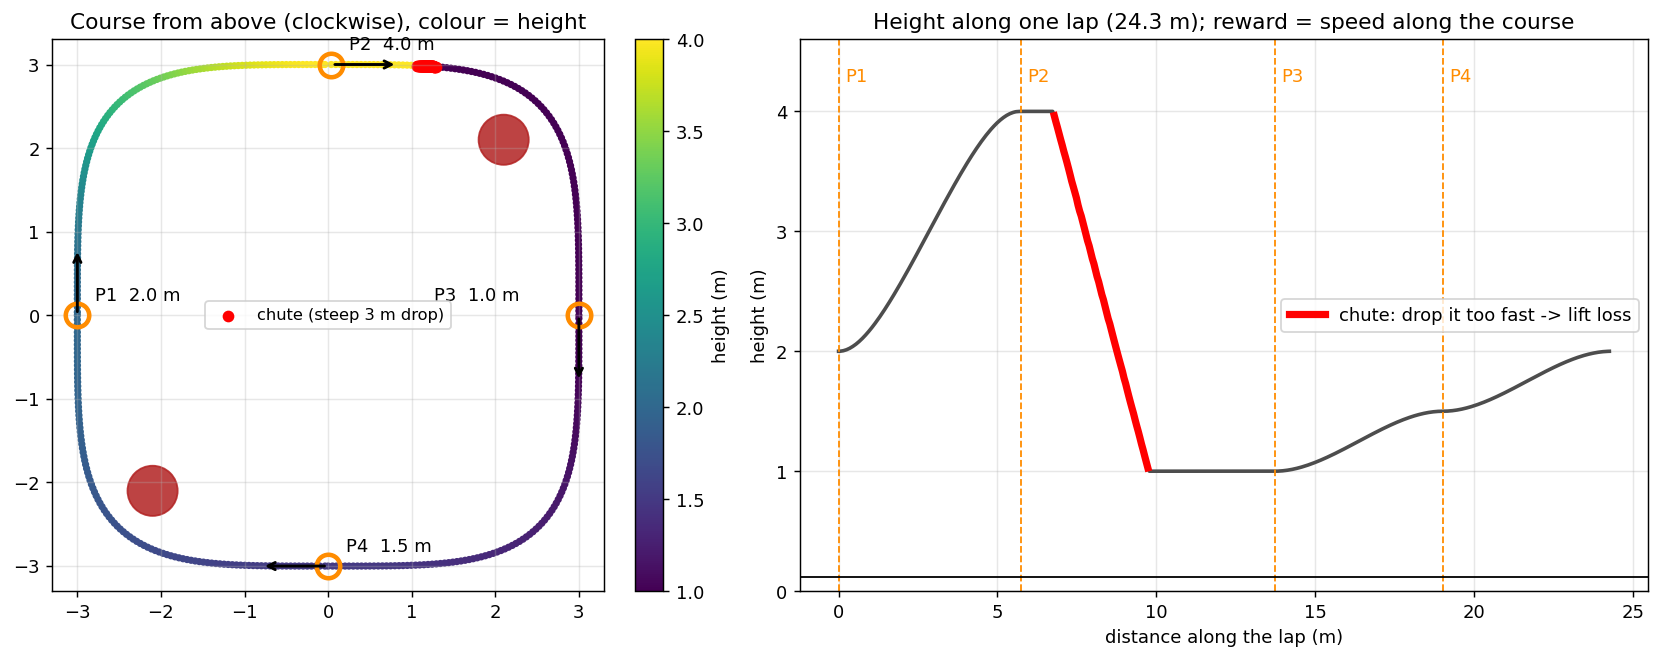
\includegraphics[width=0.63\linewidth]{figures/project/task_course.png}
    \caption{The course from above and its height profile. Red: the chute, a steep 3 m drop.}
  \end{figure}
  \vspace{-0.4em}
  \begin{columns}[T]
    \begin{column}{0.49\textwidth}
      \begin{itemize}\small
        \item A quadrotor in MuJoCo flies laps through \textbf{4 gates} (2, 4, 1 and 1.5 m high) around
              \textbf{2 pillars}.
        \item One lap is 24.3 m; a flight lasts \textbf{10 s} (500 steps).
      \end{itemize}
    \end{column}
    \begin{column}{0.49\textwidth}
      \begin{itemize}\small
        \item \textbf{4 actions}, 50 times per second (acceleration x and y, climb, turn), through an on-board
              stabiliser; \textbf{27 observations}.
        \item \textbf{Reward}: speed along the racing line. A crash costs 500 and ends the flight.
      \end{itemize}
    \end{column}
  \end{columns}
\end{frame}

% ── II.3 ──────────────────────────────────────────────────────────────────────────────────────────
\begin{frame}{Noise and the Chute Trap}
  \begin{columns}[T]
    \begin{column}{0.5\textwidth}
      \begin{figure}
        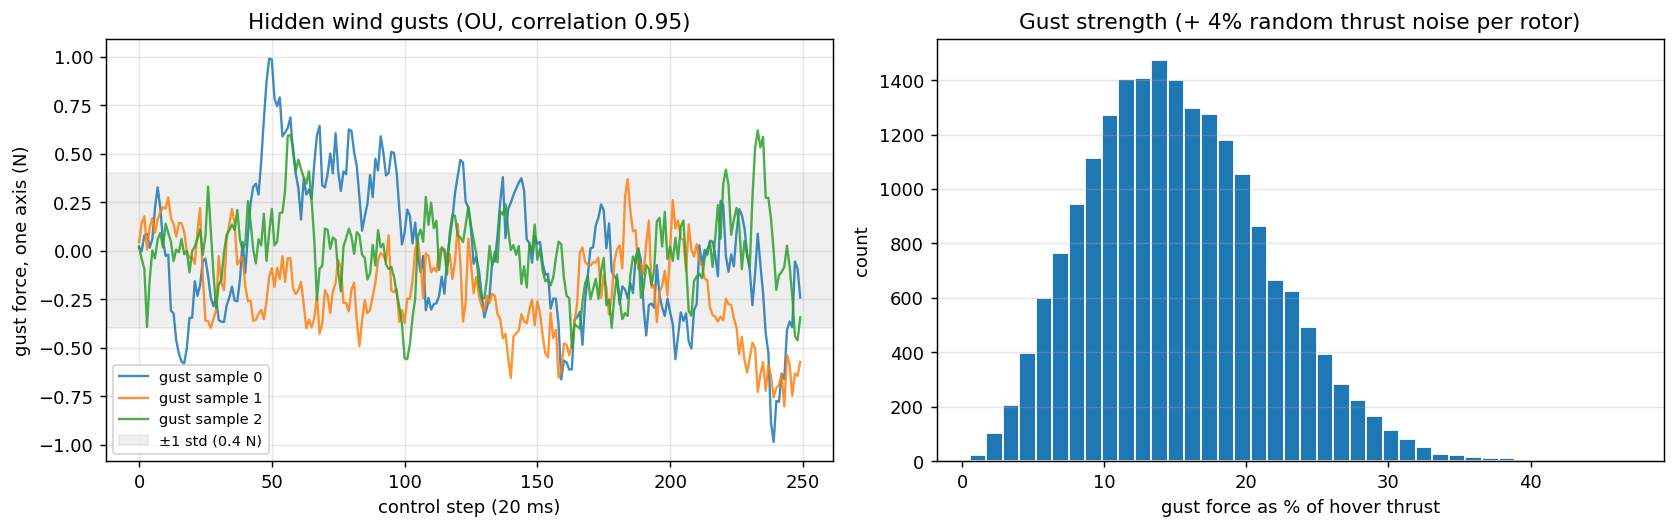
\includegraphics[width=\linewidth]{figures/project/task_wind.png}
        \caption{Hidden gusts: three samples over 5 s, and their strength.}
      \end{figure}
      \vspace{-0.5em}
      \textbf{Noise}: MACURA should \textbf{not} stop for it
      \begin{itemize}\footnotesize
        \item Hidden gusts (typically 10--20\% of the hover thrust) and 4\% noise on each rotor.
        \item Visible: a steady wind and a package of random weight (0--0.2 kg).
        \item Exploration as in the paper: pink noise for MACURA, none for MBPO and M2AC, SAC samples its policy.
      \end{itemize}
    \end{column}
    \begin{column}{0.48\textwidth}
      \begin{figure}
        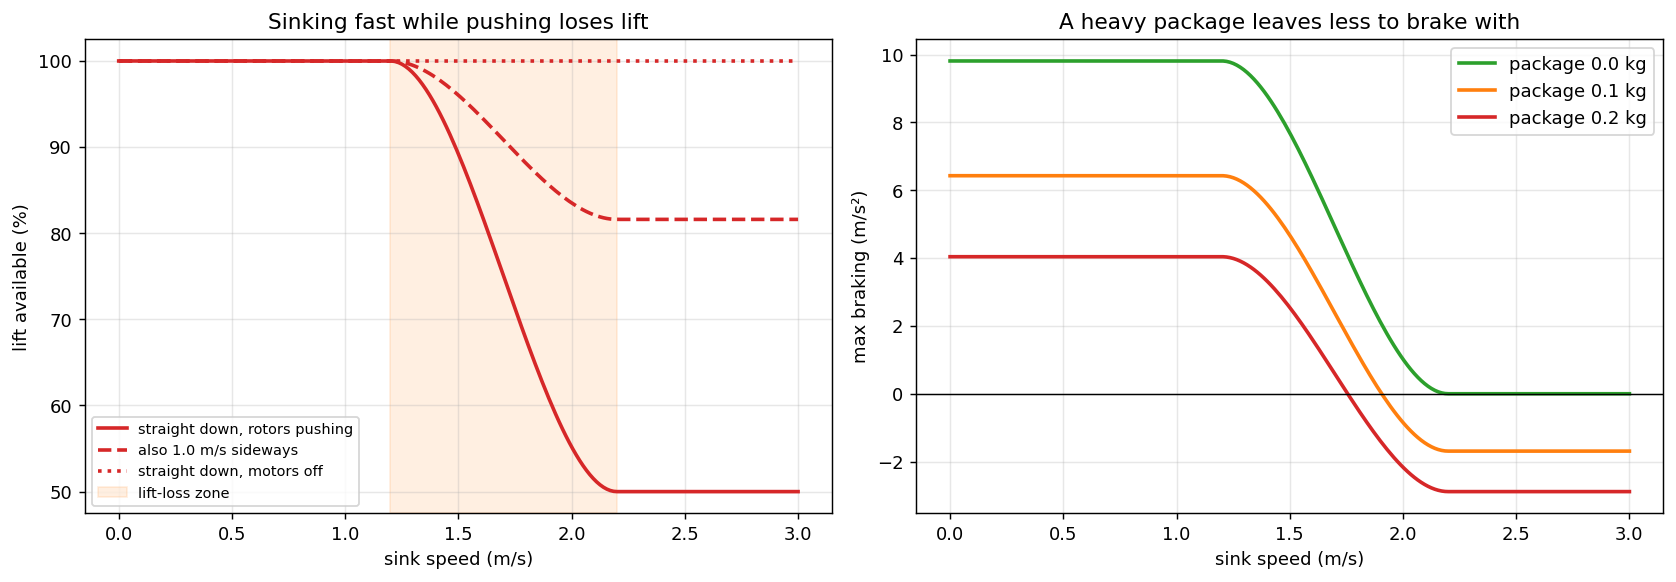
\includegraphics[width=\linewidth]{figures/project/task_lift_loss.png}
        \caption{Sinking fast while pushing loses lift.}
      \end{figure}
      \vspace{-0.5em}
      \textbf{The chute}: where the networks \textbf{should} disagree
      \begin{itemize}\footnotesize
        \item Sinking faster than \textbf{1.2 m/s} while upright and pushing loses up to \textbf{50\%} of the lift, so
              the drone cannot brake and crashes.
        \item This is rare in the data and hard to predict: exactly where MACURA should \textbf{stop imagining}.
      \end{itemize}
    \end{column}
  \end{columns}
\end{frame}

\section{II \textperiodcentered{} Method}

% ── II.4 ──────────────────────────────────────────────────────────────────────────────────────────
\begin{frame}{Implementation: One Loop, Three Rollout Rules}
  \begin{columns}[T]
    \begin{column}{0.55\textwidth}
      \scriptsize
      \begin{algorithmic}
        \For{step $=1,\dots,50{,}000$}
          \State $a\gets$ random (first 5,000) or \chg{explore$(\pi,s)$} \Comment{noise per method}
          \State $s',r\gets$ env.step$(a)$;\ add to $\Denv$
          \If{model-based \textbf{and} step mod 250 $=0$}
            \State train\_ensemble$(\Denv)$;\ $s_0\gets$ 25,000 real states
            \If{MACURA}
              \State \chg{trips $\gets$ macura\_rollout$(s_0)$}
              \State \chg{$G\gets$ gradient\_steps$(|\Dmod|)$}
            \ElsIf{MBPO}
              \State \chg{trips $\gets$ mbpo\_rollout$(s_0)$;\ $G\gets12$}
            \Else \Comment{M2AC}
              \State \chg{trips $\gets$ m2ac\_rollout$(s_0)$;\ $G\gets12$}
            \EndIf
            \State add trips to $\Dmod$ \Comment{kept for 4 rounds}
          \EndIf
          \State $G$ SAC updates on 95\% $\Dmod$ + 5\% $\Denv$ \Comment{SAC: 1 on $\Denv$}
          \State every 1,000 steps: evaluate, keep the best
        \EndFor
      \end{algorithmic}
      \vspace{0.2em}
      \code{src/training/train.py: train\_one()}
    \end{column}
    \begin{column}{0.43\textwidth}
      \footnotesize
      \textbf{Where each part lives}
      \begin{itemize}
        \item the task: \texttt{envs/drone\_env.py}
        \item the ensemble: \texttt{models/ensemble.py}
        \item the three rules: \texttt{algorithms/macura.py}, \texttt{mbpo.py}, \texttt{m2ac.py}
        \item SAC: \texttt{algorithms/sac.py}
        \item every setting: \texttt{config/config.py}
      \end{itemize}
      \textbf{Pipeline}
      \begin{itemize}
        \item 4 Kaggle GPU notebooks on 2 accounts, each training 2 algorithms $\times$ 2 seeds in parallel
              ($\approx$ 4 h).
        \item Download, then a testing notebook (50 new scenarios, plots, videos) and a live 3-D simulator.
        \item Python, PyTorch, MuJoCo, Stable-Baselines3. Runs are \textbf{deterministic} for a given seed.
      \end{itemize}
    \end{column}
  \end{columns}
\end{frame}

% ── II.5 ──────────────────────────────────────────────────────────────────────────────────────────
\begin{frame}{A Fair Protocol, and How I Chose the Task}
  \small
  \begin{columns}[T]
    \begin{column}{0.5\textwidth}
      \centering\footnotesize
      \begin{tabular}{ll}
        \toprule
        \textbf{setting} & \textbf{value} \\
        \midrule
        real steps per run & 50,000 (first 5,000 random) \\
        imagined trips & 25,000 per 250 steps, $\le$10 steps \\
        SAC batch & 95\% imagined + 5\% real \\
        MACURA & $\xi=0.5$, $\zeta=0.95$, $G_{\max}=16$ \\
        MBPO & length $1\to10$, 12 updates/step \\
        M2AC & $\alpha=10^{-3}$, 12 updates/step \\
        seeds & 4, 5, 6, 7 \\
        test & 50 new scenarios (3000--3049) \\
        \bottomrule
      \end{tabular}
    \end{column}
    \begin{column}{0.48\textwidth}
      \textbf{Fair by design}
      \begin{itemize}\footnotesize
        \item \textbf{Equal compute}: 12 updates per step for MBPO and M2AC; MACURA adapts its own and averaged
              \textbf{10.9}.
        \item The best checkpoint is chosen on other scenarios (100--119): \textbf{nothing is tuned on the test}.
        \item IQM over seeds, plus \textbf{paired} seed-by-seed comparisons (same scenarios, wind and gusts).
      \end{itemize}
      \textbf{How I chose the task}
      \begin{itemize}\footnotesize
        \item Landing tasks and a first race failed; race2 was learnable, but MACURA $\approx$ MBPO.
        \item Race3 (a deadlier chute) was kept only if MACURA beat MBPO in at least 3 of 4 seeds (0--3): a
              \textbf{rule fixed in advance}. It passed.
        \item Then the final study on \textbf{new seeds} 4--7.
      \end{itemize}
    \end{column}
  \end{columns}
\end{frame}

\section{II \textperiodcentered{} Results}

% ── II.6 ──────────────────────────────────────────────────────────────────────────────────────────
\begin{frame}{Result 1 (H1): MACURA Learns Fastest}
  \begin{figure}
    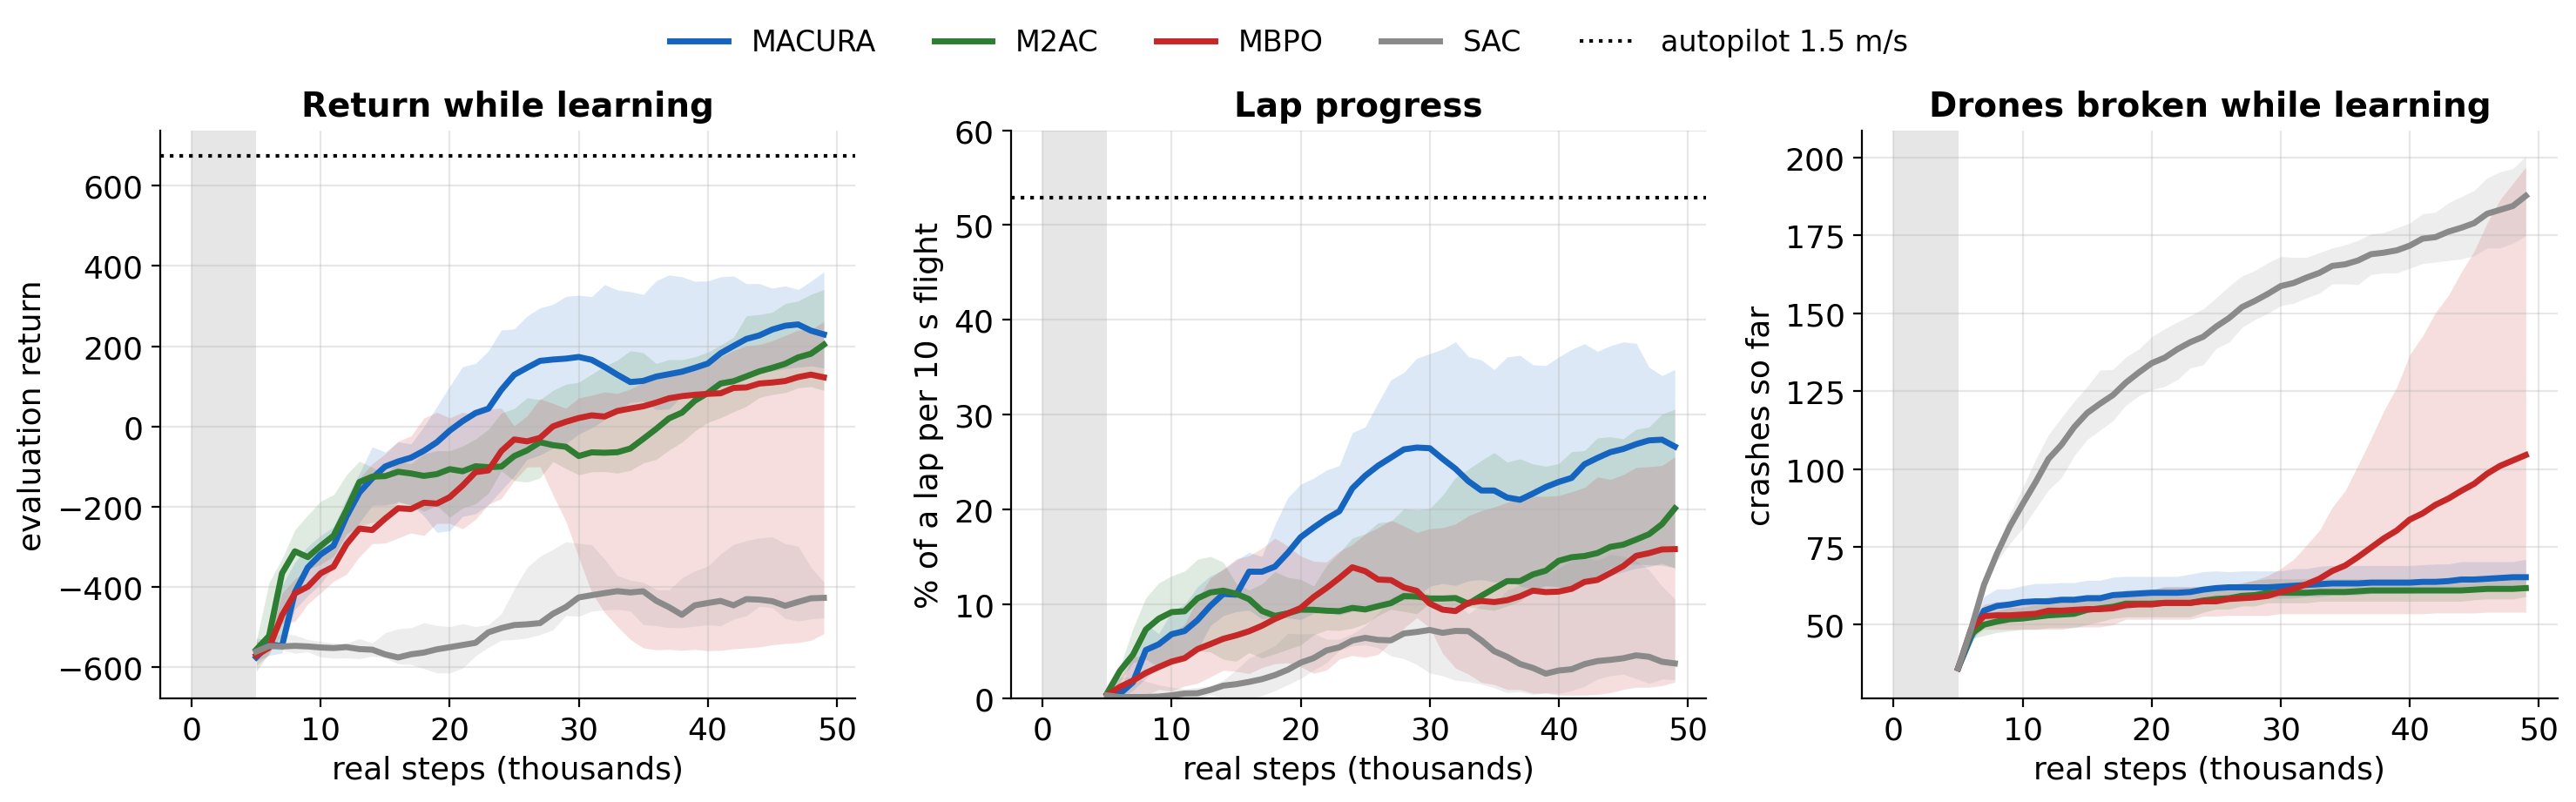
\includegraphics[width=\linewidth]{figures/project/slide_learning.png}
  \end{figure}
  \vspace{-0.3em}
  \begin{columns}[T]
    \begin{column}{0.32\textwidth}
      \footnotesize\textbf{Return}: MACURA is ahead from about 17k steps to the end; SAC is far behind.
    \end{column}
    \begin{column}{0.32\textwidth}
      \footnotesize\textbf{Lap progress}: MACURA flies the largest share of a lap (dotted: a hand-written
      autopilot).
    \end{column}
    \begin{column}{0.32\textwidth}
      \footnotesize\textbf{Drones broken}: the same for the model-based methods until MBPO's seed 5 collapses after
      30k; SAC breaks by far the most.
    \end{column}
  \end{columns}
  \vspace{0.3em}
  \centering\scriptsize IQM over seeds 4--7, 95\% CI shaded, grey = random warm-up.
\end{frame}

% ── II.7 ──────────────────────────────────────────────────────────────────────────────────────────
\begin{frame}{Result 2 (H1): Best on New Scenarios}
  \begin{figure}
    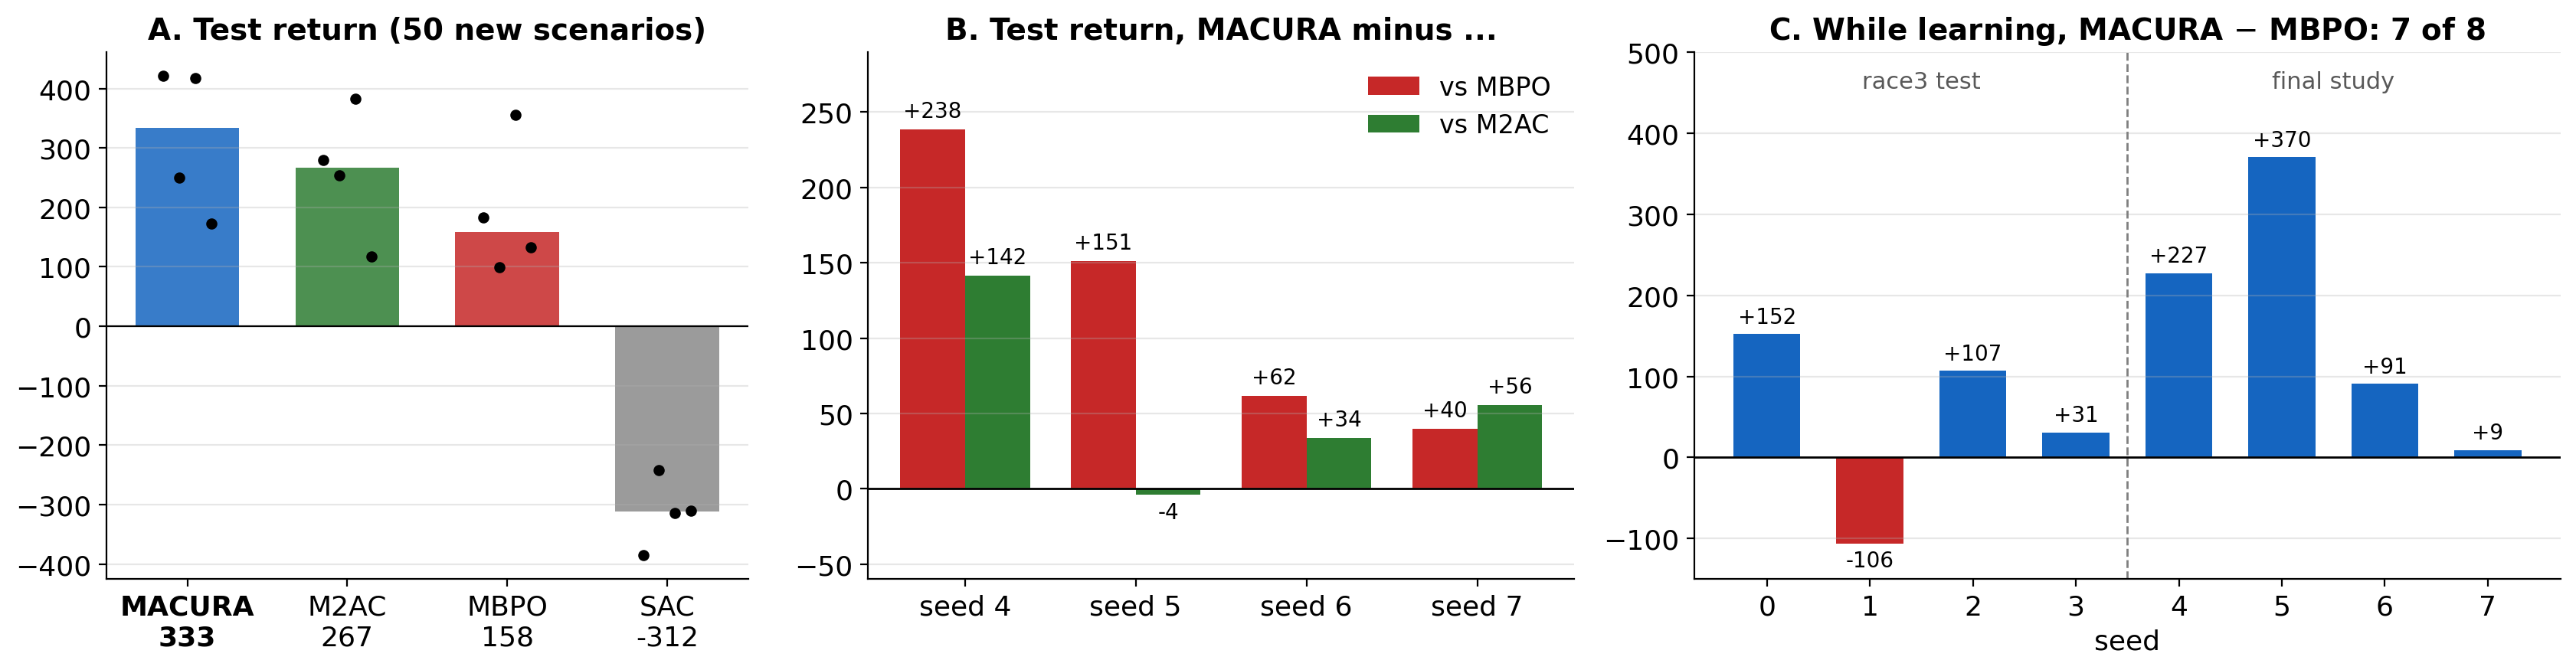
\includegraphics[width=0.96\linewidth]{figures/project/slide_results.png}
  \end{figure}
  \vspace{-0.3em}
  \begin{columns}[T]
    \begin{column}{0.4\textwidth}
      \centering\footnotesize
      \begin{tabular}{lcc}
        \toprule
        & \textbf{lap progress} & \textbf{crash rate} \\
        \midrule
        \textbf{MACURA} & \textbf{31\%} & 4\% \\
        M2AC & 24\% & 6\% \\
        MBPO & 22\% & \textbf{2\%} \\
        SAC & 7\% & 35\% \\
        \bottomrule
      \end{tabular}
    \end{column}
    \begin{column}{0.58\textwidth}
      \begin{itemize}\footnotesize
        \item \textbf{A}: the best test return (bars = IQM, dots = seeds).
        \item \textbf{B}: better than MBPO in 4 of 4 seeds, and than M2AC in 3 of 4.
        \item \textbf{C}: with the earlier seeds 0--3, better than MBPO in \textbf{7 of 8} ($p=0.035$).
        \item MBPO crashes least, but it also flies the least far.
      \end{itemize}
    \end{column}
  \end{columns}
\end{frame}

% ── II.8 ──────────────────────────────────────────────────────────────────────────────────────────
\begin{frame}{Result 3 (H2): Less Trust in the Chute}
  \begin{figure}
    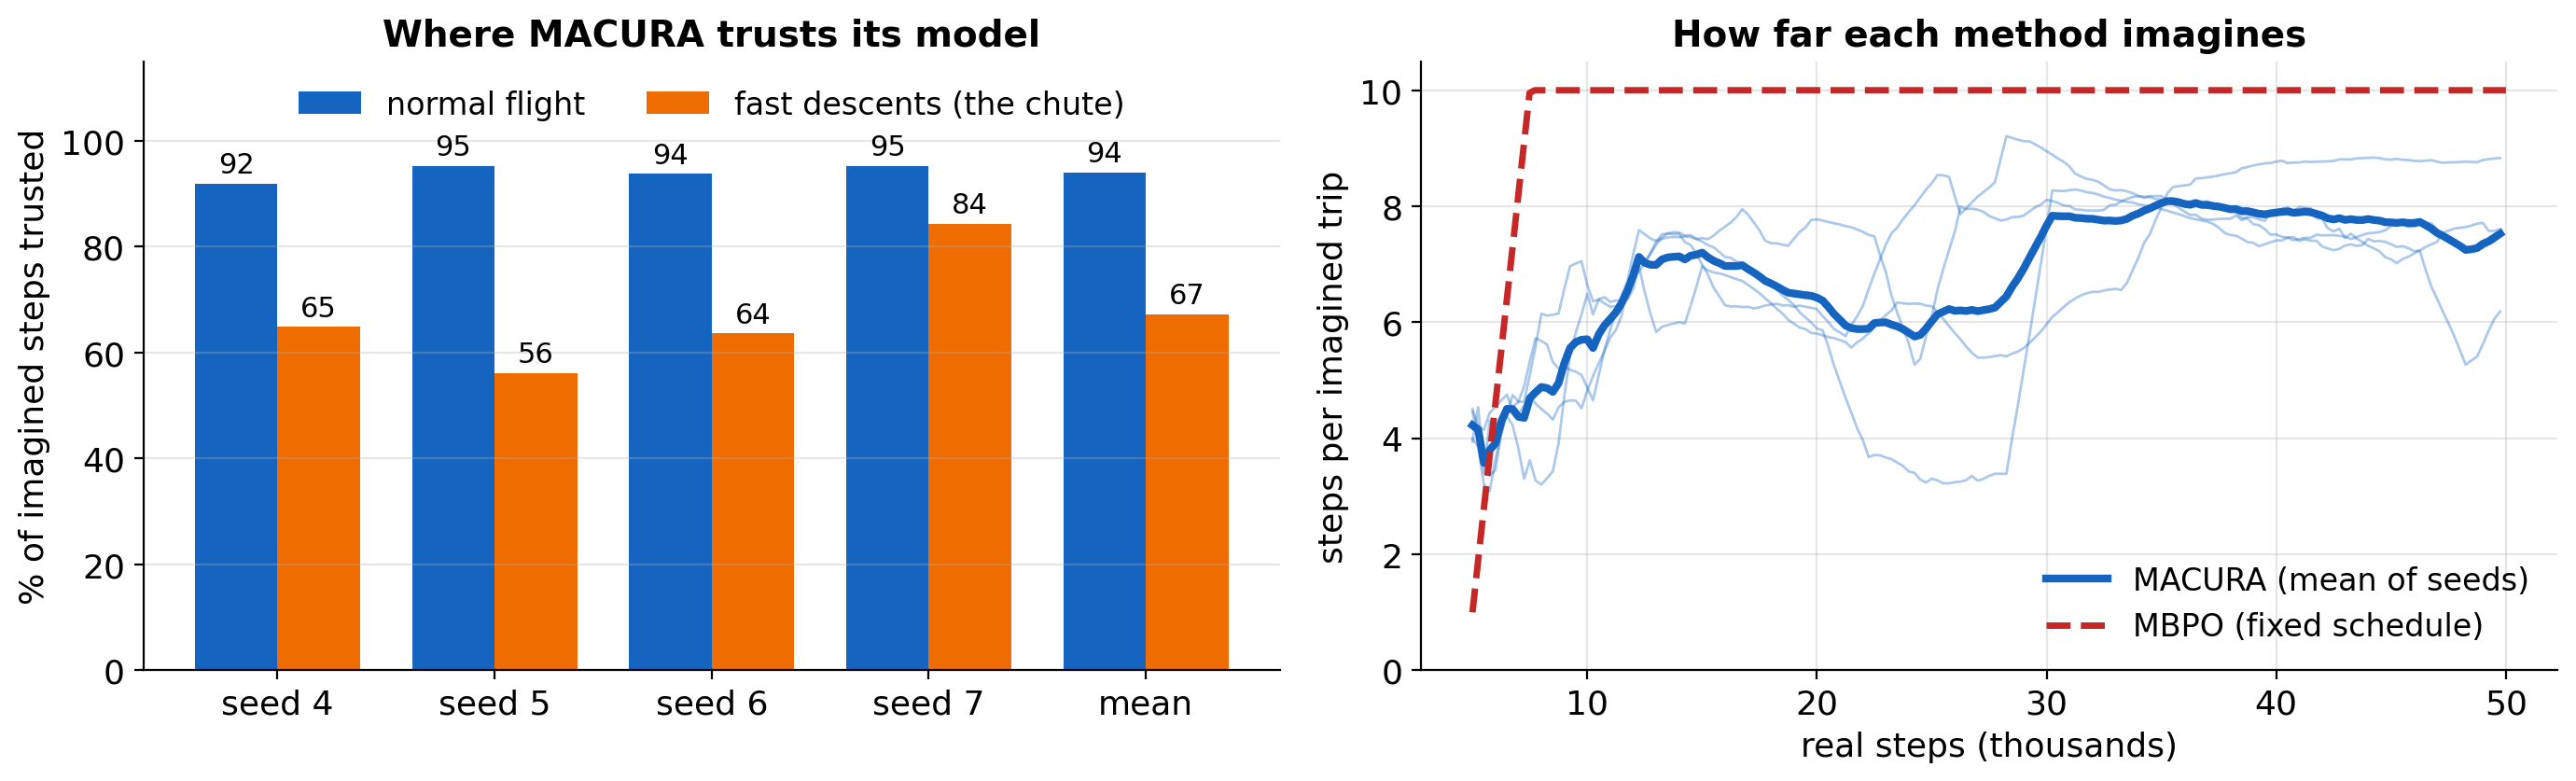
\includegraphics[width=0.94\linewidth]{figures/project/slide_trust.png}
  \end{figure}
  \vspace{-0.3em}
  \begin{itemize}\small
    \item \textbf{Left}: MACURA trusts \textbf{94\%} of its imagined steps in normal flight but only \textbf{67\%} in
          fast descents, in every seed. It notices where its model is unreliable.
    \item \textbf{Right}: its trips grow from 4 to about 8 steps as the model improves; MBPO always imagines 10.
    \item On real flights, the steps it would not trust have a \textbf{higher real error} (0.24 vs 0.21; with MBPO's model
          0.34 vs 0.20): the signal works, but it is \textbf{noisy}.
  \end{itemize}
\end{frame}

% ── II.9 ──────────────────────────────────────────────────────────────────────────────────────────
\begin{frame}{Result 4 (H2): What Each Method Trains On}
  \begin{figure}
    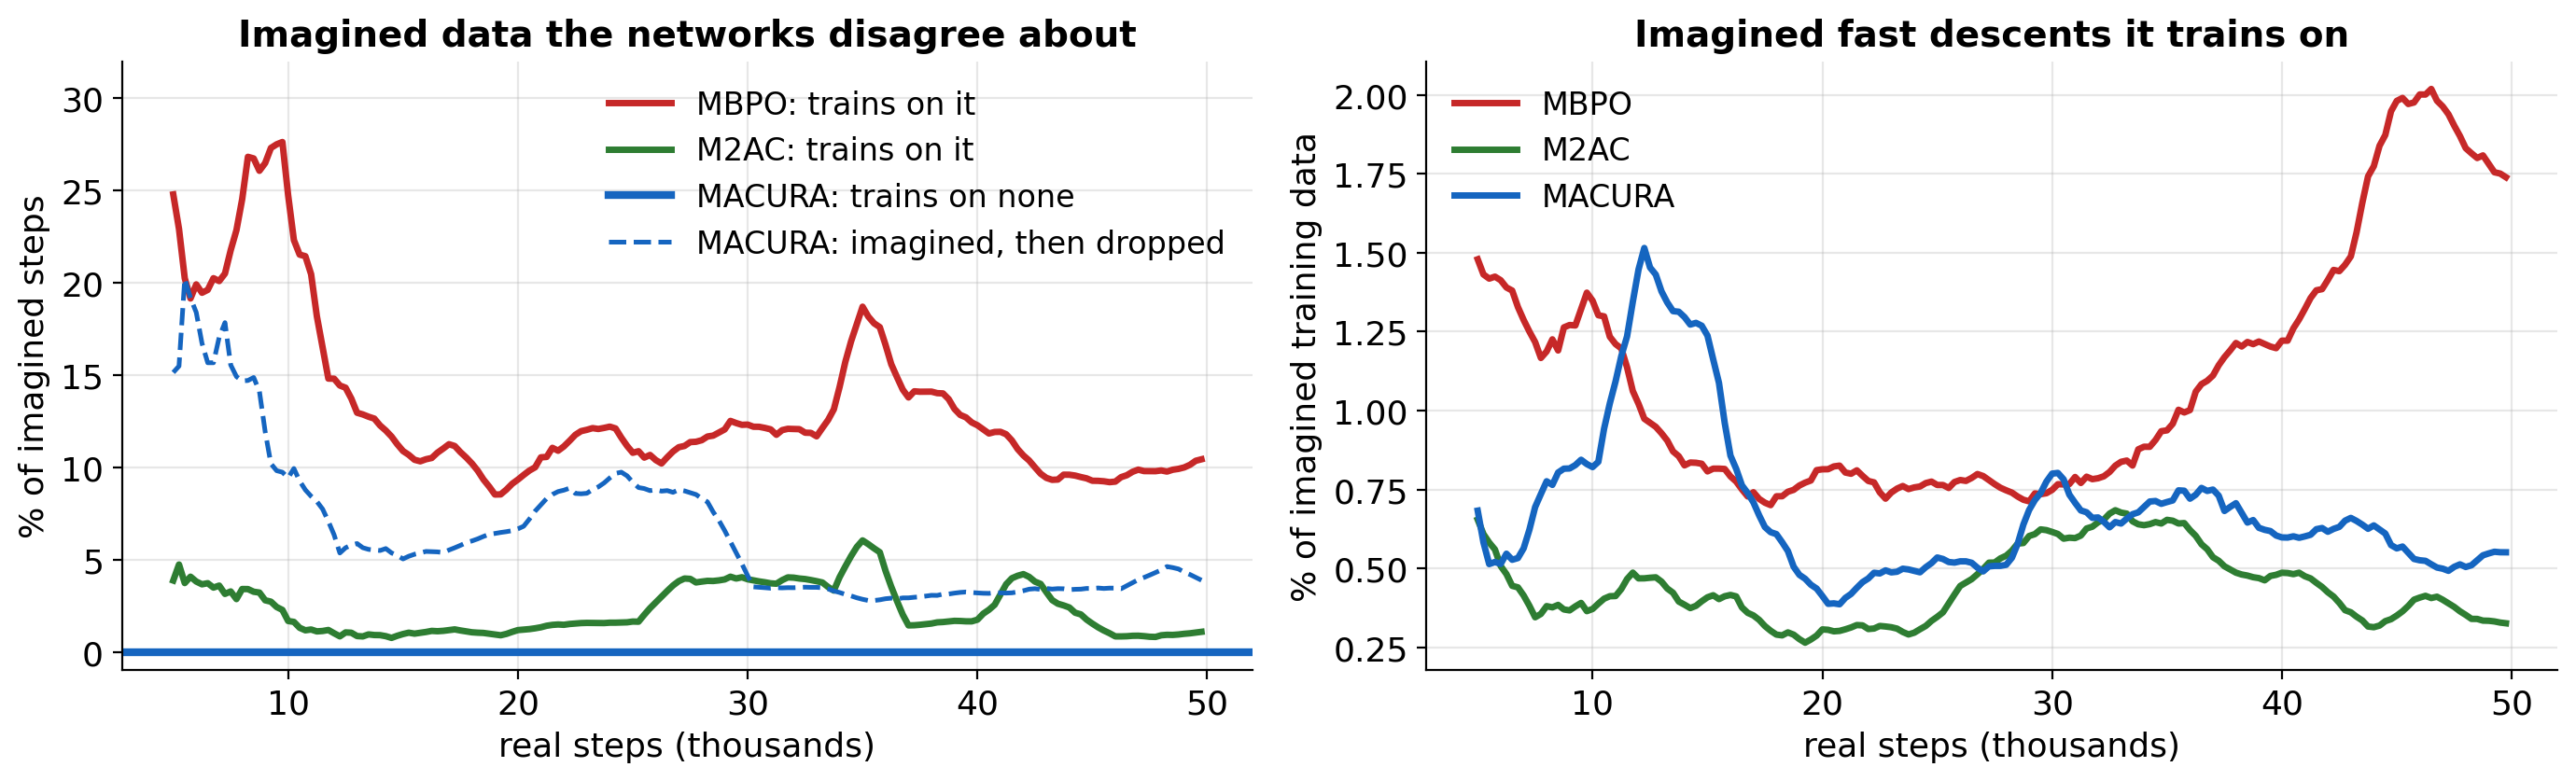
\includegraphics[width=0.94\linewidth]{figures/project/slide_untrusted.png}
  \end{figure}
  \vspace{-0.3em}
  \begin{itemize}\small
    \item \textbf{Left}: MBPO trains on \textbf{10--25\%} imagined data its own networks disagree about, M2AC on
          1--6\%, and \textbf{MACURA on none}: it imagines them, then drops them (dashed line).
    \item \textbf{Right}: late in training, MBPO trains on more and more imagined \textbf{fast descents} (up to 2\%),
          the region where its model is least reliable.
  \end{itemize}
  \centering\scriptsize Disagreement measured with MACURA's rule for every method; mean over seeds 4--7.
\end{frame}

% ── II.10 ─────────────────────────────────────────────────────────────────────────────────────────
\begin{frame}{Result 5: One Test Flight, Four Drones}
  \begin{figure}
    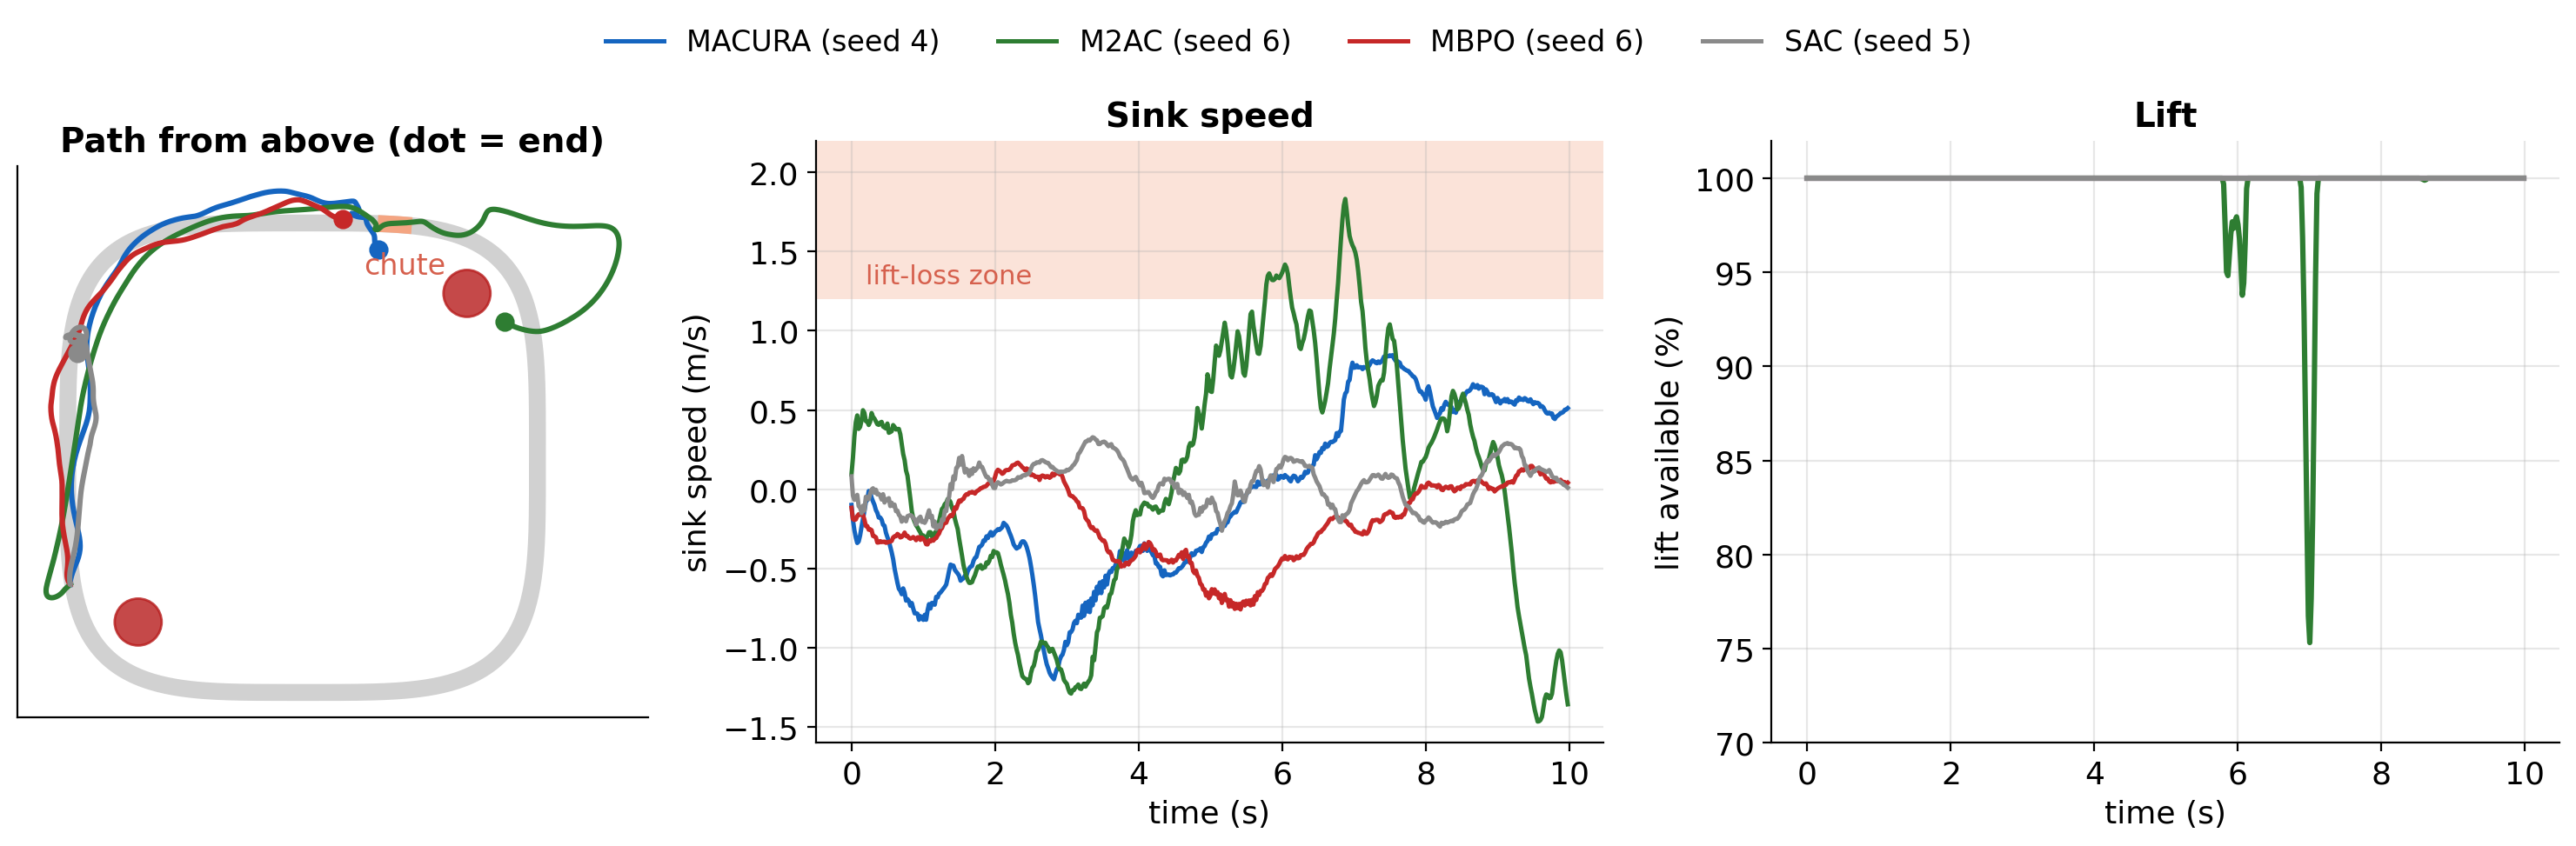
\includegraphics[width=0.9\linewidth]{figures/project/slide_flight.png}
  \end{figure}
  \vspace{-0.3em}
  \begin{columns}[T]
    \begin{column}{0.49\textwidth}
      \begin{itemize}\small
        \item \textbf{MACURA} flies furthest, reaches the chute and goes down at 0.5--0.8 m/s: its \textbf{lift stays
              at 100\%}.
        \item \textbf{M2AC} dives at up to \textbf{1.8 m/s}, enters the lift-loss zone and \textbf{loses up to 25\%}
              of its lift: the trap in action.
      \end{itemize}
    \end{column}
    \begin{column}{0.49\textwidth}
      \begin{itemize}\small
        \item \textbf{MBPO} is slower and only just reaches the top; \textbf{SAC} barely leaves the start.
        \item This is one example (scenario 3000, best seed of each), not a statistic: in the 50-scenario test the
              drones rarely sink that fast.
      \end{itemize}
    \end{column}
  \end{columns}
\end{frame}

\section{II \textperiodcentered{} Wrap-up}

% ── II.11 ─────────────────────────────────────────────────────────────────────────────────────────
\begin{frame}{Limitations}
  \begin{columns}[T]
    \begin{column}{0.49\textwidth}
      \textbf{Training budget and statistics}
      \begin{itemize}\small
        \item Only \textbf{50,000 real steps} per run, against 125k--400k in the paper. The curves are still
              rising, so I compare \textbf{early learning}, not final performance.
        \item The task is \textbf{not solved}: 31\% of a lap per 10 s, while a simple autopilot reaches 54\%.
        \item Kaggle's limits (12 h per session, about 30 GPU hours per week) did not allow longer runs.
        \item \textbf{4 seeds} per algorithm (8 for MACURA vs MBPO): a consistent result, but only at the edge of
              significance, and no hyperparameter search.
      \end{itemize}
    \end{column}
    \begin{column}{0.47\textwidth}
      \textbf{Fairness and the task}
      \begin{itemize}\small
        \item Only MACURA uses \textbf{pink noise} (the paper's protocol), so part of its gain may come from
              exploration.
        \item MBPO's schedule was not tuned for my task.
        \item \textbf{One task}, designed and changed by me five times. The rule fixed in advance and the new seeds
              reduce this risk.
        \item The drones \textbf{rarely reach the chute trap}, and the disagreement predicts the real error only
              weakly.
        \item \textbf{Simulation only}.
      \end{itemize}
    \end{column}
  \end{columns}
\end{frame}

% ── II.12 ─────────────────────────────────────────────────────────────────────────────────────────
\begin{frame}{Conclusion and Next Steps}
  \begin{columns}[T]
    \begin{column}{0.32\textwidth}
      \textbf{The paper}
      \begin{itemize}\footnotesize
        \item Trust the model only \textbf{where it trusts itself}.
        \item Imagined trips stop at the first uncertain step (GJS $\ge\kappa$).
        \item $\kappa$ and $G$ tune themselves; one knob, $\xi$.
        \item GJS reacts to disagreement, not to noise.
      \end{itemize}
    \end{column}
    \begin{column}{0.34\textwidth}
      \textbf{My project}
      \begin{itemize}\footnotesize
        \item \textbf{H1 supported}: the best test return (333 vs 267, 158 and $-312$), better than MBPO in
              \textbf{7 of 8} seeds, and no collapse.
        \item \textbf{H2 partly}: less trust in fast descents (67\% vs 94\%) and no training on data the networks
              disagree about; but the signal is noisy and the chute is rarely reached.
        \item With 50k steps: \textbf{consistent early-learning evidence, not yet proof}.
      \end{itemize}
    \end{column}
    \begin{column}{0.3\textwidth}
      \textbf{Next steps}
      \begin{itemize}\footnotesize
        \item Train longer (100k--200k steps), so the chute matters.
        \item 10 or more seeds.
        \item The same exploration for all methods.
        \item Tune $\xi$.
        \item Fly the best policies on a real drone.
      \end{itemize}
    \end{column}
  \end{columns}
\end{frame}

\begin{frame}[plain]
  \vfill\centering
  {\usebeamerfont{title}\color{black}Thank you for your attention!\par}
  \vspace{1em}
  {\small Code, results and videos: \texttt{github.com/silvergjeka22/macura-drone}}
  \vfill
\end{frame}

\end{document}
